%!TEX TS-program = xelatex
%!TEX encoding = UTF-8 Unicode
\documentclass[manuscript,screen,review]{acmart}

\setcopyright{none}
\copyrightyear{2026}
\acmYear{2026}
\acmJournal{TOSEM}
\settopmatter{printacmref=true, printccs=true, printfolios=true}
\setcitestyle{numbers,sort&compress,square}

\usepackage{amssymb,amsthm}
\usepackage{mathtools}
\usepackage{calc}
\usepackage{enumitem}
\usepackage{longtable}
\usepackage{array}
\usepackage{listings}
\usepackage{pifont}

\setlength{\emergencystretch}{3em}
\lstset{
  breaklines=true,
  breakatwhitespace=true,
  basicstyle=\ttfamily\small,
  frame=none,
  columns=fullflexible
}

\title[Semantic Mutation Score for MR Adequacy]{A Semantic Mutation Metric for Metamorphic-Relation Adequacy in Scientific Computing Programs}

\author{Meng Li}
\orcid{0000-0002-1074-1502}
\email{mlemon@usc.edu.cn}
\affiliation{%
  \institution{School of Computing, University of South China}
  \city{Hengyang}
  \country{China}
}
\affiliation{%
  \institution{Hunan Engineering Research Center of Software Evaluation and Testing for Intellectual Equipment}
  \city{Hengyang}
  \country{China}
}
\affiliation{%
  \institution{CNNC Key Laboratory on High Trusted Computing}
  \city{Hengyang}
  \country{China}
}

\author{Xiaohua Yang}
\orcid{0000-0002-2977-1787}
\email{xiaohua1963@foxmail.com}
\affiliation{%
  \institution{School of Computing, University of South China}
  \city{Hengyang}
  \country{China}
}

\author{Jie Liu}
\orcid{0009-0008-1970-8347}
\email{jieliu@usc.edu.cn}
\affiliation{%
  \institution{School of Computing, University of South China}
  \city{Hengyang}
  \country{China}
}

\author{Shiyu Yan}
\orcid{0000-0001-7626-5185}
\email{yanshiyu@usc.edu.cn}
\affiliation{%
  \institution{School of Computing, University of South China}
  \city{Hengyang}
  \country{China}
}

\begin{CCSXML}
<ccs2012>
 <concept>
  <concept_id>10011007.10011074.10011099.10011102</concept_id>
  <concept_desc>Software and its engineering~Software testing and debugging</concept_desc>
  <concept_significance>500</concept_significance>
 </concept>
 <concept>
  <concept_id>10011007.10011074.10011099</concept_id>
  <concept_desc>Software and its engineering~Software verification and validation</concept_desc>
  <concept_significance>300</concept_significance>
 </concept>
</ccs2012>
\end{CCSXML}

\ccsdesc[500]{Software and its engineering~Software testing and debugging}
\ccsdesc[300]{Software and its engineering~Software verification and validation}

\keywords{metamorphic testing, mutation testing, semantic mutation testing, metamorphic relation adequacy, metamorphic relation assessment, scientific computing}

\begin{document}

\begin{abstract}
Metamorphic testing mitigates the test-oracle problem by checking relations among executions, but classical mutation score is defined over syntactic edits and does not say whether a metamorphic-relation set observes declared domain-semantic effects. This paper introduces Semantic Mutation Score (SMS), an MR-relative adequacy metric over an admitted universe of nonequivalent semantic mutants with explicit certificates and a degeneration path back to classical mutation score. We instantiate five semantic operator families on 12 single-output scientific-computing programs and audit the resulting 60-cell design with an SMS-to-MS proof, an AST-normalized syntactic comparison, aligned-versus-cross relation analysis, and boundary and adjoint studies. The semantic pool has 5.14% AST-normalized overlap with default first-order syntactic mutants. Aligned cells score above cross-pattern cells (Cliff's delta 0.314); a 100,000-draw PUT-cluster bootstrap gives a 95% interval of [0.045, 0.594], supporting the directional hypothesis while the pre-registered large-effect threshold remains unmet. The attribution threshold is not evaluable as registered because zero-kill cells make its per-cell share undefined. An industrial real-defect arm of reproduced, MR-detectable defects from widely used scientific-computing libraries then tests the central construct claim: a four-group mutation comparison pre-registered in the dataset protocol and a per-defect detection face show that aggregate kill-rate, semantic alignment, and real-defect detection are related but distinct constructs. SMS is therefore a construct-level diagnostic for declared semantic strata, with its construct separation supported on industrial code.
\end{abstract}

\maketitle

\section{Introduction}\label{introduction}

\subsection{Software-Engineering Motivation and Scope}\label{motivation-and-scope}

Metamorphic Testing (MT) addresses the test-oracle problem in scientific
computing software: instead of checking outputs against a known-correct
reference, MT checks metamorphic relations (MRs), invariants connecting
outputs of related inputs. While \emph{semantic mutation testing} has
been named since \citet{7a6c280d9584691800e71876c716ea229335abeb} and tooled for C \citep{dan2012smtc}
and for UML state-machine behaviour \citep{derezinska2019uml}, and while
MR-adjacent data-semantic mutation \citep{sun2016mumt,sun2024datamutation,zhu2020datamorphic,chan2024metamorphic}
and recent LLM semantic-invariance MT \citep{0fa97cc4e2a0ffb6a777669b1b541c0372fac0d2} extend the mutation target
to test data, relations, and task-level semantics, the adequacy of an MR
set against \emph{domain-specific code-level faults}, conservation laws,
monotonicity, convergence order, trajectory shape, fidelity ordering,
has lacked a backward-compatible metric tied to the classical Mutation
Score (MS) lineage. \citeauthor{d7c38286734419b52de4262c9802ebdfcf4b9447}'s \citeyearpar{d7c38286734419b52de4262c9802ebdfcf4b9447} MS is defined over syntactic
Abstract Syntax Tree (AST) mutations and does not capture these domain
semantics. Recent Large Language Model (LLM) generated mutants \citep{tip2025llmorpheus,humbatova2021deepcrime} do
produce semantically richer mutants, but do not separate the
contribution of LLM source diversity from the contribution of MR design.

Throughout this paper we use the term \emph{four representative classes
of single-output scientific computing kernels} (numeric, probabilistic,
surrogate, and machine-learning), and avoid the ambiguous
software-engineering term \emph{paradigm}. The scope of our claims is
strictly bounded to single-output float-to-float kernels: each
Program Under Test (PUT) is under 2 KB. We do not claim industrial transfer
for multi-output software in this paper.

An industrial real-defect arm then tests the same semantic
distinction developed here on reproduced defects from widely used
scientific-computing libraries: mutation kill-rate, semantic stratum
alignment, and real-defect detection are related but different
constructs. The arm strengthens the semantic-mutant argument at result
level; it is not presented as a reusable benchmark artifact. Its cases
were admitted only after defect/MR detectability verification and are
reported here at result level. Candidate mining, rejected cases,
repository tooling, and benchmark release are outside this manuscript
and remain contributions of the archived dataset it draws on.

The intended reader is a software-testing researcher or practitioner who
needs to decide whether a set of MRs is adequate for a declared semantic
risk, not a domain scientist seeking a new numerical solver or a tool
user seeking another LLM-mutant generator. The novelty is therefore the
adequacy denominator and certificate structure: SMS asks which admitted
semantic-effect fibers are observed by an MR set, while preserving the
classical mutation-score form. The practical impact is diagnostic rather
than deployment-ready automation: the metric exposes when MR design,
operator applicability, or kill attribution prevents a semantic adequacy
claim from being trusted.

\subsection{Three-layer methodological framework}\label{three-layer-methodological-framework}

We organise the contribution as a three-layer framework around
domain-semantic mutation operators.

\begin{itemize}

\item
  \textbf{Layer 1, Definitional (Section~\ref{necessary-conditions-for-semantic-mutation-layer-1}).} A mutation is \emph{semantic}
  if it satisfies at least one of three necessary conditions: (a) it
  crosses a function-call or module-import boundary, (b) it depends on
  domain knowledge for legality, or (c) it changes the algorithmic
  class. The five meta-operator classes, Conservation Erosion (CE, also
  written mut\_C), Operator Substitution (OS, mut\_M), Hyperparameter
  (HP, mut\_G), Trajectory Flip (TF, mut\_T), and Structural Injection
  (SI, mut\_F), specialise these conditions across the four PUT classes.
\item
  \textbf{Layer 2, Operational (Section~\ref{equivalence-judgement-e1-e2-layer-2}, Section~\ref{mutant-pool-prescreen-and-equivalence-detection}).} An equivalence judgement
  E1 $\wedge$ E2, where E1 is Automated Verification Pipeline (AVP) coherence
  and E2 is output equivalence on K\_eq = 1000 samples, gives the
  conservative instantiation of the Layer-1 conditions. The trade-off
  against E1-alone and E2-alone variants is in Appendix A.3.
\item
  \textbf{Layer 3, Applied (Section~\ref{p2-vs-syntactic-mutants-12-put-empirical-layer-3}).} AST-normalised empirical
  traceability across all 12 PUTs: comparing 292 v4 mutants against
  1,250 cosmic-ray syntactic mutants, we show empirically that the v4
  pool is not a subset of the syntactic-mutant pool.
\end{itemize}

The 60-cell empirical audit reported in Section~\ref{statistical-analysis-and-empirical-results} stress-tests this
backbone. SMS is positioned as a strict generalisation of classical MS:
under the
degenerate limit $L = L_{\mathrm{equiv}} \wedge L_{\mathrm{killed}} \wedge L_{\mathrm{mut}}$
formalised in Section~\ref{sms-ms-degeneration-formal-statement}, SMS reduces to MS outside a
characterised exception set of pathological inputs. Layer 1 and
Layer 3 correspond to the two leading research questions, RQ1
(constructibility and backward compatibility) and RQ2 (syntactic
unreachability); the 60-cell demonstration answers RQ3--RQ5.

The empirical evidence has four roles. The 12-PUT audit is the main
stress test of the SMS construction. The AST audit tests whether the
semantic-mutant space is reachable by default first-order syntactic
mutation. The boundary and adjoint arms map when strong MRs do, and do
not, detect semantic effects. The industrial real-defect arm checks whether
the construct distinctions remain visible on verified MR-detectable defects.
These parts should be read in sequence: the theory defines the metric,
the 12-PUT audit stress-tests one empirical instantiation, the boundary
and adjoint arms test the strong-MR duality, and the industrial arm
checks whether the same construct separation appears outside synthetic
mutants and outside author-written kernels.
Table~\ref{tab:claim-evidence-map} states the licensed and unlicensed
readings of each evidence block.

\begin{table}[t]
\caption{Evidence-to-claim map for the empirical argument.}
\label{tab:claim-evidence-map}
\centering
\small
\begin{tabular}{p{0.24\linewidth}p{0.35\linewidth}p{0.33\linewidth}}
\toprule
Claim supported & Evidence used & Claim not made \\
\midrule
SMS is backward-compatible with classical MS & Formal SMS-to-MS
degeneration under the syntactic limit & SMS replaces classical mutation
score in ordinary syntactic settings \\
Semantic mutants occupy a different admitted universe & 5.14\%
AST-normalised overlap with default first-order syntactic mutants;
HP, SI, and TF are absent from the default first-order pool & Default
syntactic mutation tools can never generate higher-order semantic
mutants \\
MR alignment is visible but bounded & Aligned mean SMS 0.213 vs
cross mean SMS 0.077 under the frozen primary convention; Cliff's
\(\delta=0.314\), with PUT-cluster 95\% CI [0.045, 0.594], is positive
but below the pre-registered large-effect threshold & The current 12-PUT audit proves
a large universal aligned-vs-cross effect \\
SMS carries formal soundness, window, and attribution guarantees &
Interval-soundness, detection-window, and gap-attribution theorems
(Sections~\ref{theory-fibers}--\ref{theory-gap}) with an independent
formal audit & The idealised theorem premises hold for the empirical
pool; the exactness-defect audit \(\xi\) quantifies the deviation \\
SMS exposes adequacy boundaries & H1--H3 failures, the not-evaluable H4
estimand, zero-mass cells,
root-cause labels, the exactness-defect audit, and strong-boundary
false-positive / false-negative
cases & Failed thresholds are treated as empirical success criteria \\
Real-defect behaviour is distinct from aggregate kill-rate & The
industrial real-defect arm: a pre-registered four-group mutation
comparison plus a per-defect detection face on reproduced library
defects & The manuscript contributes a reusable
real-defect benchmark \\
\bottomrule
\end{tabular}
\normalsize
\end{table}

Table~\ref{tab:claim-evidence-map} also marks the paper's non-claims. We do not claim that SMS
is universally superior to classical MS, that pattern-derived MRs
dominate all generic relations, that higher-order mutation has been
refuted, that the industrial real-defect arm is a benchmark contribution, or that
the reported SMS values define industrial acceptance thresholds.

Figure~\ref{fig:framework} summarises the three layers and their evidence
interfaces.
\begin{figure}
\centering
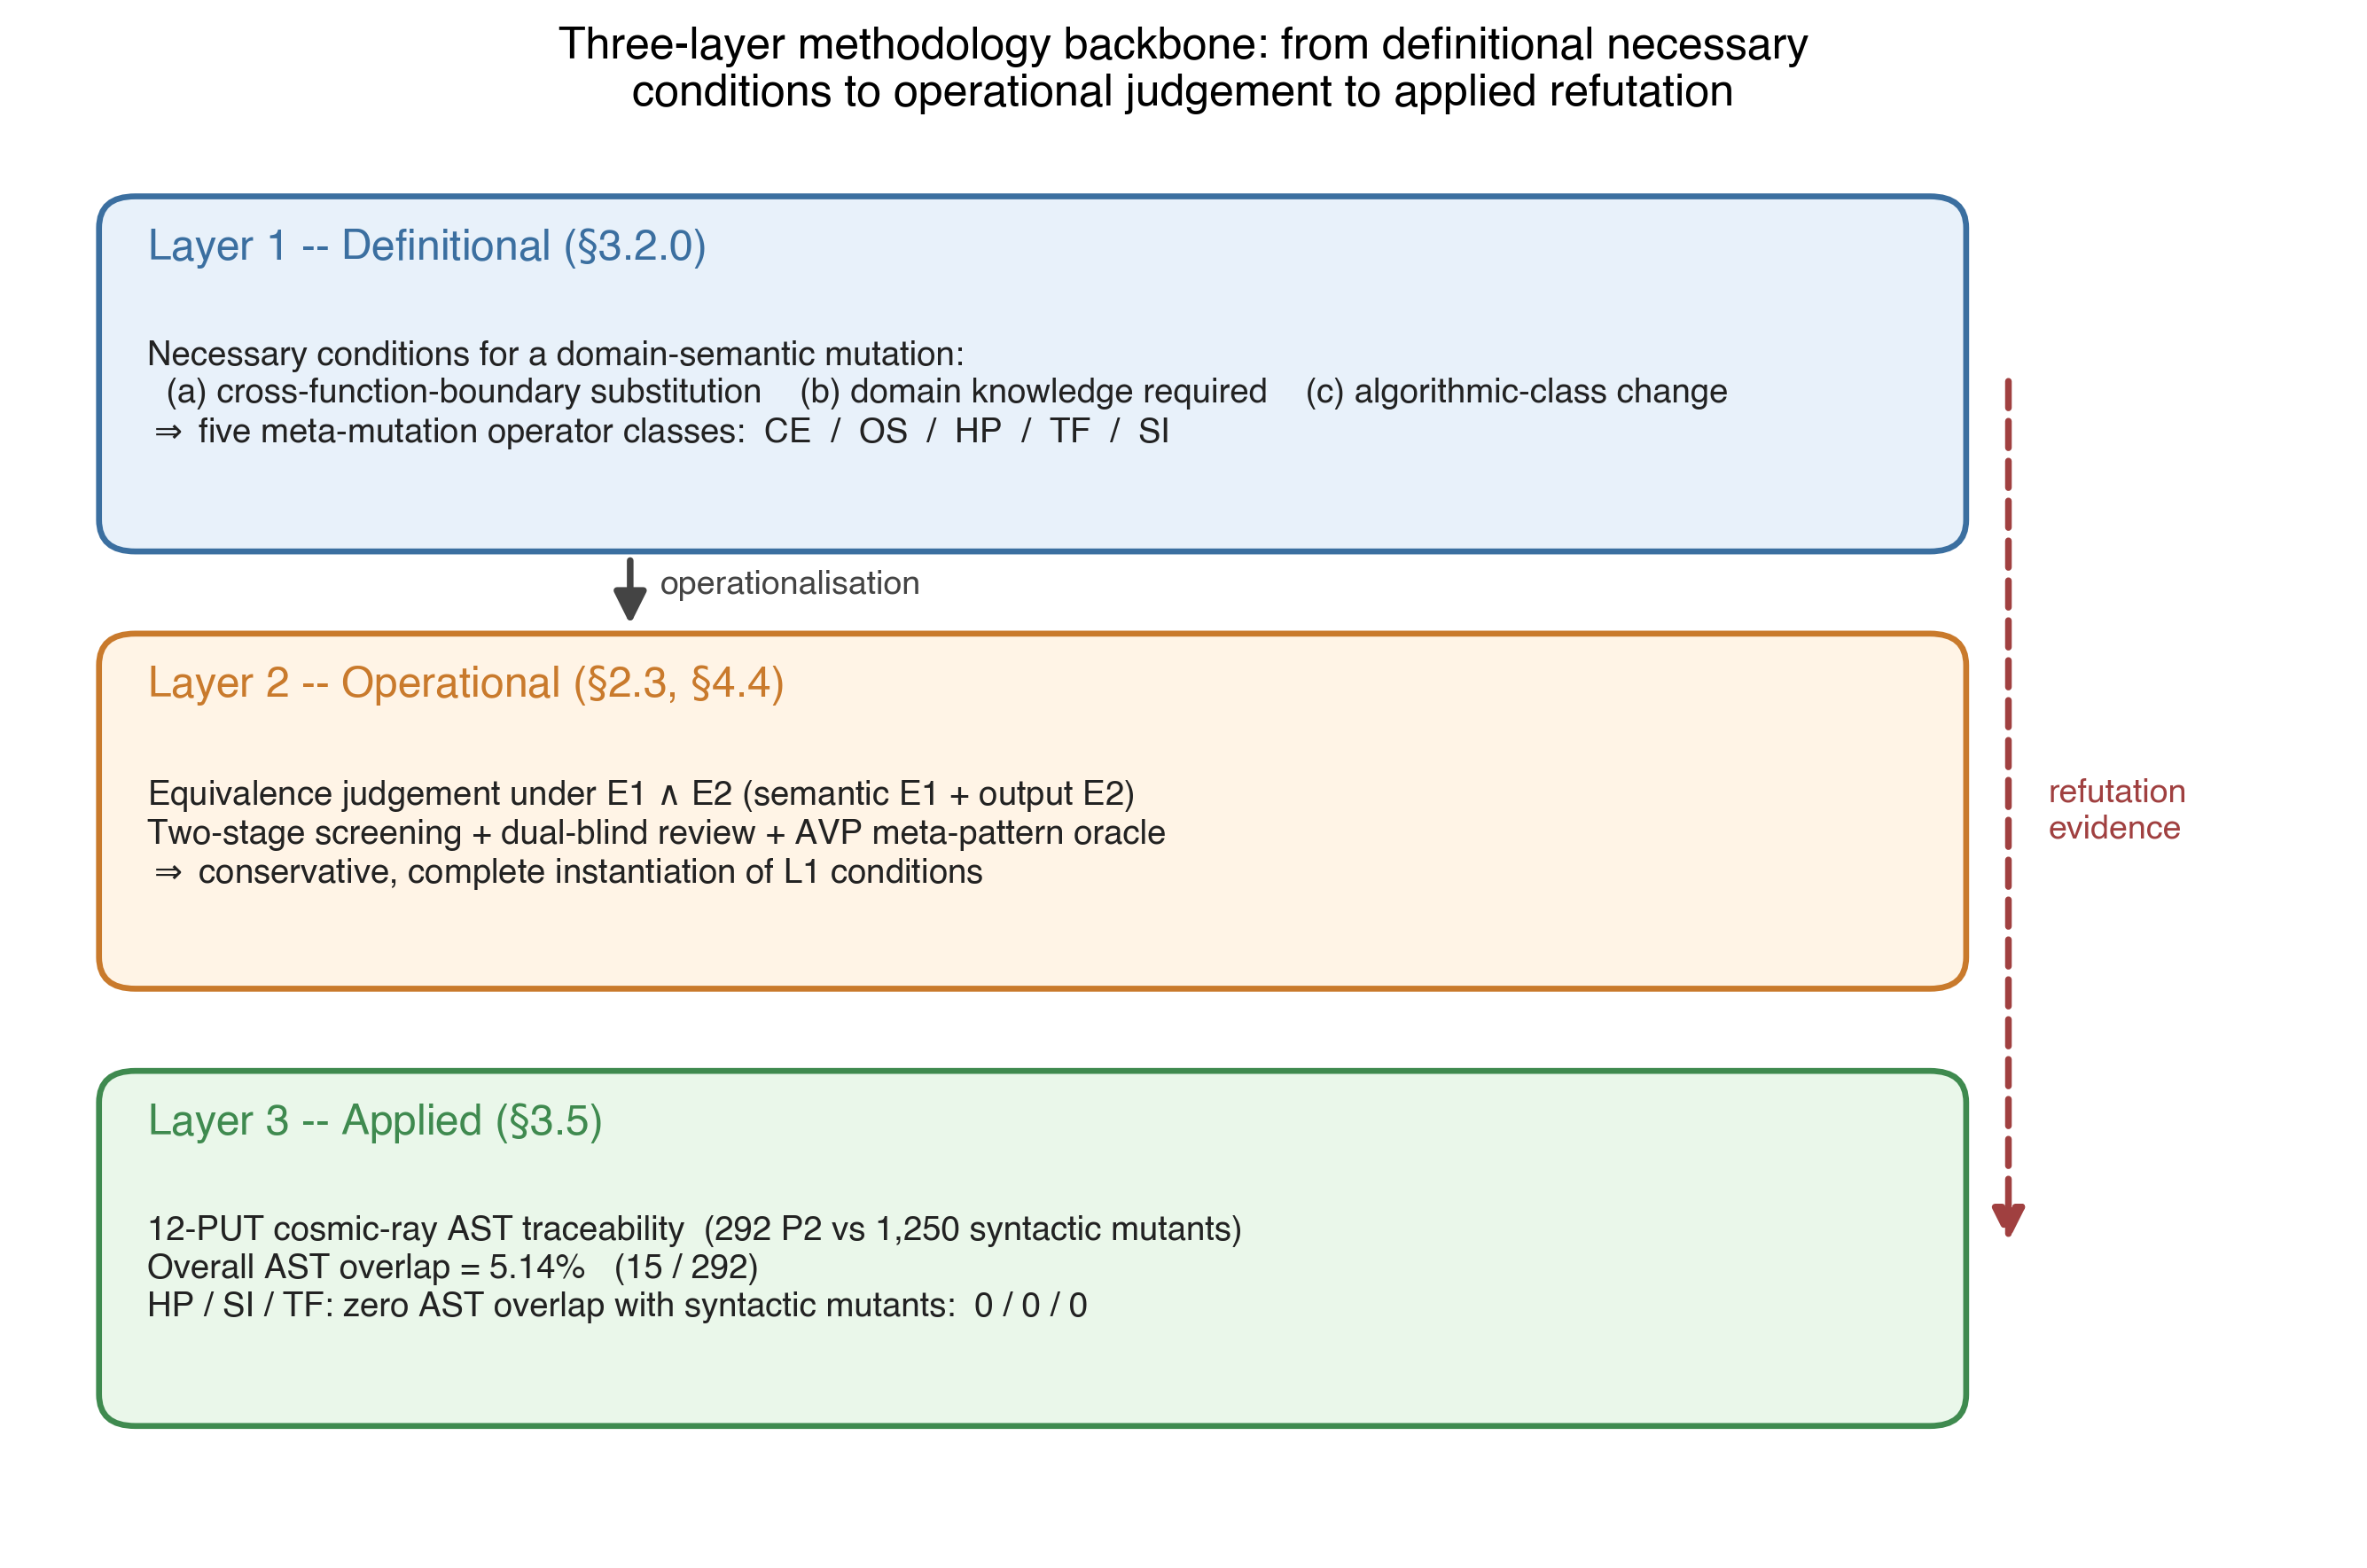
\includegraphics[width=0.85\linewidth,height=\textheight,keepaspectratio]{figures/png/fig1_three_layer_methodology.png}
\Description{Three stacked layers connect definitional conditions for semantic mutation, the operational E1-and-E2 judgement, and the applied AST-normalised audit across 12 programs under test.}
\caption{Three-layer methodological framework: Layer 1 (definitional
necessary conditions), Layer 2 (operational \(E_1 \wedge E_2\)
judgement), Layer 3 (applied AST-normalised traceability across 12
PUTs).}\label{fig:framework}
\end{figure}

\section{Related Work}\label{related-work-and-roadmap}

Seven lines of prior work bracket the contribution of this paper.

General MT foundations and surveys define the oracle-problem setting and
the role of metamorphic relations in paired-test reasoning
\citep{chen2018metamorphic,segura2016survey,liu2014alleviate}. Because
our empirical subject class is scientific computing, we also take the
scientific-software testing survey by \citet{kanewala2014scientific} as
the nearest domain background.

\textbf{(a) Classical mutation testing.} \citet{d7c38286734419b52de4262c9802ebdfcf4b9447} and
\citet{d461ab9482b7fb5eadd7e6cd2c6dffced8ede8b8} survey syntactic mutation. The Coupling Effect
Hypothesis (CPH), that tests detecting simple faults also detect complex
faults, underpins the use of MS as a fault proxy \citep{demillo1978hints,andrews2005mutation,just2014mutants}. We
argue in Section~\ref{p2-vs-syntactic-mutants-12-put-empirical-layer-3} that CPH holds within syntactic mutation but does not
automatically extend across the syntactic-versus-domain-semantic
boundary, even when it couples simple syntactic faults to complex
syntactic faults. The Section~\ref{p2-vs-syntactic-mutants-12-put-empirical-layer-3} empirical evidence (5.14\% AST overlap on 12
PUTs, with HP, SI, and TF at 0/0/0) is the empirical witness for this
boundary. The connection between correctness notions and test evidence
also precedes modern mutation-score practice \citep{budd1982correctness};
SMS inherits that concern but changes the adequacy object from a program
test set to an MR set over admitted semantic mutants.

\textbf{(b) Higher-order mutation.} \citet{c03829bdd1a6e45113092384bf0fa05a064ca54a} and \citet{kintis2018effective}
study compositions of first-order syntactic mutants. We
explicitly exclude any equivalence claim about Higher-Order Mutation
(HOM) and list HOM equivalence as a residual threat (Appendix F.2).

\textbf{(c) LLM-generated mutants.} \citet{tip2025llmorpheus}
introduce LLMorpheus, which uses single-LLM JavaScript mutants.
\citet{humbatova2021deepcrime} introduce DeepCrime for
deep-learning real-fault mutation. \citet{dakhel2024llm} extend
LLM-driven mutation testing to test generation on Java PUTs, providing
an \emph{Information and Software Technology} anchor for the LLM-mutant
lineage. To our knowledge no prior LLM-mutant work isolates \emph{LLM
source diversity} from \emph{MR design} in the contribution to effect
size; the three-stage ablation in Section~\ref{cross-source-v4-protocol-summary} closes this gap. On the
equivalent-mutant problem, \citet{delgadoperez2020equivalent} emphasise
the importance of the \texttt{equiv} term in the MS denominator; we
extend that classical bitwise-equivalence definition to a semantic-class
equivalence E1 $\wedge$ E2 in Section~\ref{equivalence-judgement-e1-e2-layer-2}. \citet{zhang2021classintegration} demonstrate MT
validation in class-integration test ordering, a
non-scientific-computing domain, and the present paper specialises MT to
scientific-computing PUTs and couples it to a domain-semantic mutation
operator framework.

\textbf{(d) Semantic mutation operators across testing communities.}
Semantic mutation as a research line is older than the LLM-mutant
lineage. \citet{7a6c280d9584691800e71876c716ea229335abeb} introduce \emph{semantic
mutation testing} as a path distinct from syntactic mutation; \citet{dan2012smtc}
tool the approach for C; \citet{derezinska2019uml}
apply \emph{semantic mutation operators} to UML state-machine behaviour
by perturbing semantic-variation-point interpretations rather than
syntactic structure. Within MT specifically, \citet{sun2016mumt,sun2024datamutation}
propose \emph{data mutation operators} and the $\mu$MT methodology to drive
MR acquisition through controlled data-semantic perturbation; \citet{zhu2020datamorphic}
formalise \emph{datamorphic testing}, separating
datamorphisms (test-case-to-test-case mappings) from metamorphisms
(test-case-to-Boolean mappings) over data semantics; \citet{chan2024metamorphic}
extend generic data mutation operators to unsupervised
software-defect-prediction validation. Most recently, \citet{0fa97cc4e2a0ffb6a777669b1b541c0372fac0d2}
formalise \emph{semantic invariance} in LLM MT under paraphrase,
fact-reorder, expand/contract, and context-shift transformations. These
works establish that mutation can target data, relation, task, and
behavioural semantics. SMS adds an MR-adequacy denominator for
scientific kernels, a classical-MS limit, and an empirical map of the
tolerance-governed strong boundary.

\textbf{(e) MR adequacy and coverage.} The decisive distinction is the
counting object. Existing work counts MR or source-test obligations,
differentially executed elements, MR diversity, validity, or classical
mutant detection
\citep{xiang2019compositeMR,fu2024mtadequacy,liu2024mtcoverage,ba2025metamorphiccoverage,xie2024mutmodel,huang2022mrprioritization,zhang2022effectivemrselection}.
The non-MT semantic-coverage analogue counts specification obligations
\citep{302e9d254f138148abce2feda1319f9cb32cd914}. SMS instead counts
admitted non-equivalent domain-semantic code mutants while retaining the
classical MS form.
Table~\ref{tab:closest-denominator-comparators} makes that denominator
distinction explicit.

\begin{table}[t]
\centering
\footnotesize
\caption{Closest denominator-oriented comparators to SMS. The comparison
is by adequacy object and denominator semantics, not by whether a paper
uses the phrase metamorphic-testing adequacy.}
\label{tab:closest-denominator-comparators}
\begin{tabular}{p{0.22\textwidth}p{0.34\textwidth}p{0.34\textwidth}}
\toprule
Work & Denominator or counted object & Relation to SMS \\
\midrule
\citep{fu2024mtadequacy,liu2024mtcoverage} & MR obligations, MR coverage, and source-test obligations & Closest MR/MT adequacy comparators, but property/coverage denominators rather than semantic mutant classes \\
\citep{ba2025metamorphiccoverage} & Differentially executed code elements in paired MT runs & Execution-side coverage comparator, not MR-set semantic adequacy \\
\citep{xie2024mutmodel} & MR feature/diversity space & Boundary surrogate for MR-set quality, not an adequacy fraction over faults or semantic classes \\
\citep{huang2022mrprioritization,zhang2022effectivemrselection} & MR validity, coverage, and classical mutation-score signals & Boundary surrogate for cost-effective MR choice, not a denominator-bearing adequacy metric \\
\citep{302e9d254f138148abce2feda1319f9cb32cd914} & Semantic obligations under a specification & Non-MT semantic-coverage analogue; test-suite side rather than MR-set side \\
\bottomrule
\end{tabular}
\end{table}

\textbf{(f) Property-relative and numerical-specification mutation.}
Property-aware mutation and numerical-specification testing reject
irrelevant mutants or encode floating-point requirements
\citep{0ed19a2ecb5537dbf1c5f25a818f45a34d418ae8,525d0597f3b46f6b8dc6e0ee1e0cd507d23dc22b}.
SMS instead evaluates an MR set over five semantic fault classes and
retains the MS form.

\textbf{(g) Semantic foundations and the certificate gap.} Abstract and
approximate transformation semantics, refinement mutation, UTP, and
differential dynamic logic provide machinery for proof-bearing effects
\citep{46aba24d3e925f6d8d2efd5b5f6ee0d5ea7558cd,72269d5ab33ed790ece6856ba0309ed070d83622,11efca8804ed387c9cc3956868f0eb43597c8d10,6d492b783178b02dae163fbfe837857b982deed2,92d99528fe8e70345901cf56aa4d1037f0c3aa96,97a550b469c6151734d1220e37a7985d896191ee,7a867d014c3e10e45e4220c5dcf605e8df6ef38d}.
SMS supplies the MR-adequacy denominator and audit, but its certificates
are evidence records rather than proof objects.

\textbf{Closest comparison.} Min-MR-Complete
\citep{li2026minmrcomplete} optimises MR subsets over an admitted
mutant--draw universe; this paper constructs, scores, and audits that
universe. Neither attaches machine-checkable proof certificates.

The SMS metric is conceptually complementary to the code-verification
scope of ASME V\&V 20-2009 §3, which targets numerical-solver
correctness. SMS targets MR fault-detection adequacy; we make no
normative compliance claim (Appendix E.3 records this as a long-term
aspiration only).

\section{Problem Formulation and Semantic Mutation Model}\label{research-questions-and-hypotheses}

This section states the research questions before introducing the metric:
scope and novelty are stated as RQ1--RQ2, while RQ3--RQ5 test whether
one empirical instantiation is usable, discriminative, and consistent
enough to support the construct. The formal model then gives reviewers a
small declared vocabulary, the semantic-certificate record, and the
SMS-to-MS degeneration that ties the proposal to the mutation-testing
lineage.

\subsection{Research Questions}\label{research-questions}

The research questions run from formal measurement
scaffolding (RQ1), through structural separation (RQ2), to the
empirical demonstration on the 60-cell audit (RQ3--RQ5). RQ1 is answered
by construction and proof (Sections~\ref{theory-setting}--\ref{theory-fibers}: the undecidability theorem (Theorem~\ref{thm:undecidability}),
the fiber characterisation (Proposition~\ref{prop:fiber}), and the duality theorem (Theorem~\ref{thm:duality}), together
with the SMS--MS degeneration of Section~\ref{sms-ms-degeneration-formal-statement}); RQ2 by the
AST-normalised structural audit (Section~\ref{p2-vs-syntactic-mutants-12-put-empirical-layer-3}); RQ3--RQ5 by the pre-registered
statistical pipeline (Section~\ref{statistical-analysis-and-empirical-results}). This ordering mirrors the three-layer
framework of Section~\ref{three-layer-methodological-framework}: Layer 1 (definitional) carries RQ1, Layer 3 (applied)
carries RQ2.

\begin{itemize}

\item
  \textbf{RQ1 (Formal measurement scaffolding and guarantees).} Can semantic
  mutation be represented as certified effect fibers so that SMS
  degenerates to classical MS, strong MRs have a tolerance-bounded
  detection window, unresolved equivalence yields a sound interval, and
  score shortfall separates alignment from strength gaps
  (Theorems~\ref{thm:degeneration}, \ref{thm:window},
  \ref{thm:interval}, and~\ref{thm:gap})?
\item
  \textbf{RQ2 (Syntactic unreachability).} To what extent is the
  domain-semantic mutant space induced by the five operators reachable
  by default-configuration first-order syntactic mutation tools at the
  AST-normalised level?
\item
  \textbf{RQ3 (Instantiability).} Do the five semantic mutation
  operators instantiate a usable nonequivalent semantic-mutant
  denominator across the 60 PUT-MP cells, as reflected by
  inst\_rate, equiv\_rate, C1\_share, and survive\_rate?
\item
  \textbf{RQ4 (Discrimination, LLM-source decoupling, the strong
  boundary, and industrial construct separation).} Does SMS discriminate
  primary-stratum aligned cells ($k = k^\star(i)$, the PUT's
  class-primary meta-pattern) from
  cross cells ($k \neq k^\star(i)$); does cross-source LLM pooling under an
  identical prompt move the aligned-versus-cross effect size, or only the
  kill-set quality; where does the strong boundary of Theorem~\ref{thm:window}
  lie empirically, on which real and textbook programs does a strong
  MR kill the genuine fault, and where does the duality fail as a weak-MR
  false positive or as a surviving non-equivalent mutant; and does the
  construct separation among aggregate kill-rate, semantic alignment,
  and real-defect detection remain visible on an industrial arm of
  reproduced, MR-detectable defects from widely used
  scientific-computing libraries?
\item
  \textbf{RQ5 (Cross-class consistency).} Does the aligned-versus-cross
  SMS pattern generalise across four representative classes of
  single-output scientific-computing kernels? (The relationship between
  SMS and the coverage-style surrogate Pattern Coverage is reported
  descriptively at n = 12 as a hypothesis-generating observation, not a
  confirmatory test.)
\end{itemize}

\subsection{Hypotheses}\label{hypotheses}

The empirical questions RQ3--RQ5 carry pre-registered hypotheses; RQ1 is
answered by Theorems~\ref{thm:window}, \ref{thm:interval},
\ref{thm:gap}, and~\ref{thm:degeneration} and RQ2 by the Section~\ref{p2-vs-syntactic-mutants-12-put-empirical-layer-3} structural audit, neither of
which is a statistical hypothesis.
The hypothesis definitions, primary-MR convention, and statistical
reporting hierarchy are frozen in
\texttt{docs/experiment\_documentation/EXPERIMENT\_DESIGN.md} at commit
\texttt{0f2509527f346f9433c3cf90959bb07d80601a23} and in the Zenodo
replication package
\href{https://doi.org/10.5281/zenodo.20250664}{10.5281/zenodo.20250664}.

\begin{itemize}

\item
  \textbf{H1 (RQ3).} At least 4 of the 5 operators produce $\geq$ 5 non-equivalent
  mutants on at least 9 of the 12 PUTs.
\item
  \textbf{H2 (RQ4; pre-registered as an exploratory large-effect
  target).} The aligned-SMS to
  cross-SMS odds ratio is $\geq$ 3.0, and Cliff's $\delta$ is $\geq$ 0.474.
  The threshold was fixed before data collection. Its large-effect
  verdict follows the point estimate, while the direction is evaluated
  with a dependence-aware PUT-cluster interval
  (Section~\ref{rq2-stipulated-alternative-power}).
\item
  \textbf{H3 (RQ5).} A within-class sign test gives 4/4 across the 4 classes,
  and CV($\Delta$SMS) \textless{} 0.5.
\item
  \textbf{H4 (RQ4).} Mean suspect\_share is $\leq$ 0.20 across the 60 cells.
\end{itemize}

\textbf{What would count against the construct (stated post hoc).} The
pre-registered thresholds stress one instantiation and do not exhaust
falsifiability. The construct itself would be disconfirmed by: (i) the
degeneration path failing empirically, with SMS and MS disagreeing on
the same pools in the syntactic limit; (ii) the aligned-versus-cross
direction reversing systematically across designs; (iii) the industrial
arm showing the generic baselines' kill sets nesting the pattern-derived
kill sets, leaving no construct separation; or (iv) certificates failing
audit, with declared strata not matching observed effects. Criteria
(ii)--(iv) were observed not to occur; criterion (i) was not directly
tested and is open to replication. We state these criteria post hoc,
after the verdicts, and label them accordingly.

The 12 PUTs are deliberately \emph{Numerical Recipes}--style compact
kernels: they provide a verifiable minimum working example for the
three-layer backbone, while industrial-scale transfer is left to future
work under the representativeness threat.

% [thematic break removed]

\section{Formal Measurement Scaffolding and Guarantees}
\label{formal-measurement-scaffolding}
\label{notation-and-equivalence-judgement}

This section fixes the admitted mutant universe, equivalence states,
score denominator, and conditions under which MR kills support semantic
claims. The proof
techniques are standard---set decomposition, closure, triangle
inequalities, and classical undecidability reductions. The contribution
is their integration into an executable mutation-adequacy contract;
full proofs are kept in supplementary Appendix G.

\subsection{Vocabulary and Notation}\label{vocabulary-inheritance}

We use a small vocabulary throughout the method. The terms are declared
here before they are used in the SMS construction.

\textbf{Program Under Test (PUT).} A PUT is the scientific-computing
kernel being assessed. We write the \(i\)-th PUT as \(S_i\).
Its admitted input domain is \(\mathcal{X}_{\mathrm{adm}}\), and
\(\mathcal{D}_P\) is the sampling distribution used by bounded
equivalence checks.

\textbf{Metamorphic Relation (MR).} An MR is a property that relates the
outputs of related inputs. The MR family used for PUT \(S_i\) and
meta-pattern \(k\) is written \(\mathrm{MR}_{i,k}\).

\textbf{Meta-pattern (MP).} An MP is a semantic stratum of MR behaviour,
such as conservation, monotonicity, convergence, trajectory structure, or
fidelity order. The index \(k\) denotes the MP being tested.

\textbf{Semantic operator.} A semantic operator is a mutation family
\(\mathrm{mut}_j\) designed to perturb a declared MP. The operator index
\(j\) identifies the intended semantic effect.

\textbf{Semantic mutant.} A semantic mutant \(s'\) is a finite syntactic
edit of \(S_i\) that is admitted by semantic operator \(\mathrm{mut}_j\)
and is certified against the declared MR family. Formally,
\[
  s' \in \mathrm{mut}_j(S_i).
\]
The word semantic therefore names the certification target, not a second
editing mechanism.

\textbf{Detection set (kill set).} For an MR family \(\mathrm{MR}_{i,k}\),
the detection set is the subset of admitted semantic mutants
that the family kills:
\[
  \mathcal{K}(\mathrm{MR}_{i,k}) =
  \{s' \in \mathrm{mut}(S_i): \mathrm{killed}(s', \mathrm{MR}_{i,k})\}.
\]
Different MR families can observe different detection sets. SMS therefore
measures adequacy relative to a declared stratum; it is not a total order
over all possible MR families. (The word \emph{fiber} is reserved for
the effect-map preimages of Section~\ref{theory-fibers}: a fiber is a
property of the mutant, a detection set is a property of the MR family.)

\textbf{Evaluation unit and mutant pool.} The evaluation unit is the
(PUT, meta-pattern) cell \((i,k)\). Each PUT carries one admitted pool
\(\mathrm{mut}(S_i) = \bigcup_j \mathrm{mut}_j(S_i)\), mixing the
operator families; the same pool is evaluated against every
\(\mathrm{MR}_{i,k}\). The operator index \(j\) is a per-mutant
generation-time label (the mutant's declared fiber), not a cell axis:
per-operator scores \(\mathrm{SMS}_{i,k,j}\) are not separately
identified in this campaign because the pool is not stratified into
per-operator denominators at evaluation time. Fiber-level information
enters through the per-mutant labels, which feed the root-cause layer
and the exactness-defect audit \(\xi\) (Section~\ref{theory-gap}).

\textbf{Three-state equivalence status; killed and surviving mutants.}
The E1 $\wedge$ E2 judgement of Section~\ref{equivalence-judgement-e1-e2-layer-2} is evidence, not proof, so
each admitted mutant occupies exactly one of three states:
\texttt{CERTIFIED\_EQUIVALENT}, where a machine-checkable certificate
establishes observational equivalence (the current pipeline instantiates
no such certifier, so this state is presently empty);
\texttt{CONFIRMED\_NON\_EQUIVALENT}, where an execution witnesses an
observed-output divergence beyond $\varepsilon_{\mathrm{eq}}$ or the AVP
verdicts differ on some relation (the E1 $\vee$ E2 failure route); and
\texttt{EQUIVALENCE\_UNRESOLVED}, where E1 $\wedge$ E2 sample agreement
holds without a certificate. A confirmed non-equivalent mutant is killed
when at least one MR in \(\mathrm{MR}_{i,k}\) passes on \(S_i\) and
fails on \(s'\); killed mutants are always confirmed non-equivalent
(Lemma~\ref{lem:witness}), and a confirmed non-equivalent mutant that is
not killed is surviving. Writing \(n_{i,k}\) for the confirmed
non-equivalent count, \(\kappa_{i,k}\) for the killed count, and
\(u_{i,k}\) for the unresolved count of a cell:

\begin{align*}
\mathrm{mut}(S_i) &= \mathrm{certified}_{i,k} \cup \mathrm{killed}_{i,k} \cup \mathrm{survive}_{i,k} \cup \mathrm{unresolved}_{i,k} \quad \text{(disjoint)} \\
\mathrm{SMS}_{i,k} &:= \mathrm{SMS}^{\mathrm{strict}}_{i,k} = \frac{\kappa_{i,k}}{n_{i,k}}, \qquad
\mathrm{SMS}^{\mathrm{cons}}_{i,k} = \frac{\kappa_{i,k}}{n_{i,k} + u_{i,k}} \in [0,\,1]
\end{align*}

The reported score is the strict reading, whose denominator is the
confirmed non-equivalent population; the conservative companion divides
the same killed count by confirmed plus unresolved, treating every
unresolved survivor as truly non-equivalent
(Theorem~\ref{thm:interval} bounds the ground truth between the two).
Both are reported as \texttt{NA} when their denominator is empty. In the
audited v4 campaign the unresolved set is empty in every cell
($u_{i,k} = 0$), so the two readings coincide and equal the classical
ratio $|\mathrm{killed}|/(|\mathrm{mut}| - |\mathrm{equiv}|)$; in the v3
campaign ten cells carry 80 sample-agreement incidences that the
refinement classifies as unresolved, and all ten are zero-kill cells, so
both readings are $0$ there and no recorded number changes.

\textbf{Semantic Mutation Score (SMS).} SMS preserves the classical
Mutation Score (MS) ratio while replacing the internal definitions of
mutant generation, equivalence, and killing with MR-relative semantic
definitions. The classical concepts of mutation operator, mutant,
equivalent mutant, killed mutant, surviving mutant, and MS are inherited
from \citet{d7c38286734419b52de4262c9802ebdfcf4b9447} and
\citet{ammann2008introduction}; the three-state status refines the
classical \texttt{equiv} term without adding formula terms.

The complete notation table is in Appendix A.1; index sets and tolerance
parameters ($\varepsilon_{\mathrm{eq}}$, $\varepsilon_{\mathrm{AVP}}^k$,
$K_{\mathrm{eq}} = 1000$, $N = 20$) follow that table.

\subsection{Semantic-Operator Signatures}\label{operator-signatures}

Operator family and alignment:

\begin{align*}
\mathrm{MUT} &= \{\mathrm{mut}_C,\, \mathrm{mut}_M,\, \mathrm{mut}_G,\, \mathrm{mut}_T,\, \mathrm{mut}_F\} \quad \text{(open, extensible)} \\
\mathrm{mut}_j &: \text{Programs} \to 2^{\text{Programs}} \\
\mathrm{align}(j) &= j \quad \text{(design choice, not theorem)}
\end{align*}

The alignment map is the design-level correspondence between operator
families and the meta-patterns their intended violations feed; it labels
mutants, not cells. Cell-level slicing uses the PUT's class-primary
meta-pattern $k^\star(i)$ (Section~\ref{primary-mp-convention}): a cell
$(i,k)$ is \emph{aligned} when $k = k^\star(i)$ and \emph{cross}
otherwise.
Table~\ref{tab:p2-01} records the single mapping used throughout the
paper.

\begin{table}[t]
\caption{Operator signatures.}\label{tab:p2-01}
\centering
\begin{tabular}{@{}lll@{}}
\toprule
Operator & Failure semantics & Aligned MP \\
\midrule
mut\_C & Conservation-breaking & MP\_1 Conservation \\
mut\_M & Monotonicity-breaking & MP\_2 Monotonicity \\
mut\_G & Convergence-breaking & MP\_3 Convergence \\
mut\_T & Trajectory-distorting & MP\_4 Trajectory \\
mut\_F & Fidelity-order-breaking & MP\_5 Partial-order \\
\bottomrule
\end{tabular}
\end{table}

Per-PUT specialisation tables (mut\_C/M/G/T/F across 12 PUTs and 4
classes) are deferred to \textbf{Appendix B.2}.

\subsection{Equivalence Judgement}\label{equivalence-judgement-e1-e2-layer-2}

The equivalence judgement is the executable instantiation of the Layer-1
necessary conditions (Section~\ref{necessary-conditions-for-semantic-mutation-layer-1}). For each candidate mutant
\texttt{s\textquotesingle{}}:

\begin{itemize}

\item
  \textbf{E1 (AVP-coherent):} $\forall$ mr $\in \mathrm{MR}_{i,k}$: $\mathrm{AVP}(S_i, mr)$ =
  $\mathrm{AVP}(s', mr)$.
\item
  \textbf{E2 (Output-equivalent):} $\forall$ x in $K_{\mathrm{eq}}=1000$ samples
  $\sim \mathcal{D}_P$: $\|S_i(x) - s'(x)\| \leq \varepsilon_{\mathrm{eq}}$.
\end{itemize}

E1 $\wedge$ E2 makes false equivalence require both checks to mis-pass;
one failure routes the mutant to confirmed non-equivalence. For a
per-sample disagreement probability at least \(p_0\), E2's miss
probability is at most
\((1-p_0)^{K_{\mathrm{eq}}}\leq e^{-K_{\mathrm{eq}}p_0}\).
Sample agreement without a certificate remains unresolved. Appendix A.3
compares E1-only and E2-only alternatives; Appendix G gives the
classical limit.

\paragraph{Semantic certificate record.}
The empirical certificate records PUT, operator and stratum identifiers,
edit and invariant classes, E1/E2 evidence, kill vector, LRCA labels,
generation source, review status, and artifact trace. It is an auditable
record, not a proof object. Only confirmed non-equivalent mutants enter
the strict denominator; LRCA never filters it.

The killed determination preserves the classical OR-aggregation:

\[
\begin{aligned}
\mathrm{killed}(s', \mathrm{MR}_{i,k}) \iff{} & \exists\,mr \in \mathrm{MR}_{i,k}: \\
& \mathrm{AVP}(S_i, mr) = \text{pass} \wedge
  \mathrm{AVP}(s', mr) = \text{fail}.
\end{aligned}
\]

\subsection{Root-Cause Diagnostic Layer}\label{lrca-engineering-attribution-layer-descriptive-not-in-sms}

LRCA annotates kills as C1 likely semantic, C2 tolerance, C3 OOD, C4
statistical-assumption, or C5 artefact, with priority
C5 \(>\) C4 \(>\) C3 \(>\) C2 \(>\) C1. It reports
\texttt{C1\_share} and \texttt{suspect\_share}; both are \texttt{NA} on
zero-kill cells and neither changes SMS. LRCA classifies kill mechanism,
whereas \(\xi\) compares the generation label with the checker stratum,
so a C1 kill may still be off-fiber. Appendix A.2 contains the full
decision tree.

\subsection{Backward-compatibility declaration}\label{backward-compatibility-declaration}

SMS retains the classical
\(\lvert\mathrm{killed}\rvert/
(\lvert\mathrm{mut}\rvert-\lvert\mathrm{equiv}\rvert)\) structure
\citep{d7c38286734419b52de4262c9802ebdfcf4b9447}. Only the internal
definitions of generation, equivalence, and killing change. Under
Theorem~\ref{thm:degeneration}, those definitions and the three-state
refinement collapse to classical syntactic mutation, behavioural
equivalence, and same-input difference detection; Corollary~\ref{cor:lrca}
then trivialises LRCA. The interface is fixed while the operator,
meta-pattern, and diagnostic inventories remain extensible.

\subsection{Degeneration to Classical Mutation Score}\label{sms-ms-degeneration-formal-statement}

The Section~\ref{backward-compatibility-declaration} backward-compatibility claim is formalised as a degeneration
theorem. The full notation cross-reference is \textbf{Appendix G.1}; the joint
conditions are in \textbf{Appendix G.2}, the lemma proofs in
\textbf{Appendix G.3}, and the full theorem proof in \textbf{Appendix G.4}. We
state only the main theorem and corollary here; the three construction
lemmas are stated and proved in the supplementary material as
Lemma G.1--G.3.

\textbf{Definition (Degenerate limit).}
$L = L_{\mathrm{equiv}} \wedge L_{\mathrm{killed}} \wedge L_{\mathrm{mut}}$, where each joint
condition is a pair of paired axes acting on one layer of the SMS
formula:

\begin{itemize}

\item
  $L_{\mathrm{equiv}} = L1 \wedge L2$: $\varepsilon_{\mathrm{eq}} \to 0 \wedge K_{\mathrm{eq}} \to \infty$ (controls equiv
  layer; Lemma G.1).
\item
  $L_{\mathrm{killed}} = L3 \wedge L4$: $\varepsilon_{\mathrm{AVP}} \to 0 \wedge$ relation set =
  $\{\mathrm{MR}_{\mathrm{eq}}^{S_i}\}$, the reference-anchored identity
  relation: identity source transformation ($r = \mathrm{id}$), output
  relation $R(y,y') \equiv y = y'$, with the follow-up output compared
  against the recorded reference output of the original program $S_i$
  (controls killed layer; Lemma G.2).
\item
  $L_{\mathrm{mut}} = L5 \wedge L6$: $\mathrm{mut}_j$ switches to rule-based syntactic
  operators (Mothra-style, or modern MutMut/PIT-style) $\wedge$ PUT class $\subseteq$ imperative deterministic
  programs (controls mut layer; Lemma G.3).
\end{itemize}

The same conjunction admits an orthogonal regrouping that separates what
tends to a limit from what is merely switched: write
$L_{\mathrm{lim}} = L1 \wedge L2 \wedge L3$
($\varepsilon_{\mathrm{eq}} \to 0$, $K_{\mathrm{eq}} \to \infty$,
$\varepsilon_{\mathrm{AVP}} \to 0$) for the quantitative limit axes, and
$L_{\mathrm{switch}} = L4 \wedge L5 \wedge L6$ (reference-anchored
identity relation; rule-based syntactic operators; imperative
deterministic PUT class) for the discrete configuration switches. Then
$L = L_{\mathrm{lim}} \wedge L_{\mathrm{switch}} = L_{\mathrm{equiv}} \wedge L_{\mathrm{killed}} \wedge L_{\mathrm{mut}}$:
the same conjunction under two readings, the lemma-facing pairing above
and the limit/switch split used to state Theorem~\ref{thm:degeneration}.

\begin{theorem}[SMS $\to$ MS degeneration]\label{thm:degeneration}
Fix the switch component $L_{\mathrm{switch}}$ and assume
$\mathrm{supp}(\mathcal{D}_P) \supseteq \mathcal{X}_{\mathrm{adm}}$ (the
sampling distribution's support covers the admitted input domain). Along
the limit component $L_{\mathrm{lim}}$, outside the exception set
$\mathcal{N}_{\mathrm{exc}}$ of Lemma G.1 (over floating-point, finite,
input domains: the finite set of pathological inputs, empty in the exact
discrete case; under the continuum idealisation: a
$\mathcal{D}_P$-measure-zero set),

\[ \mathrm{SMS}_{i,k} \xrightarrow{L_{\mathrm{lim}}} \mathrm{MS}_{i} = \frac{|\mathrm{killed}_{i}^{\mathrm{classic}}|}{|\mathrm{mut}^{\mathrm{syntax}}(S_i)| - |\mathrm{equiv}_{i}^{\mathrm{classic}}|} \]

where the right-hand side is the classical Mutation Score of
\citet{d7c38286734419b52de4262c9802ebdfcf4b9447} over the pooled syntactic-mutant set,
$\mathrm{killed}^{\mathrm{classic}}$ is the same-input
difference-detection set,
$\mathrm{equiv}^{\mathrm{classic}}$ is the behavioural-equivalence set,
and $\mathrm{mut}^{\mathrm{syntax}}$ is the syntactic-mutant set; the
per-operator-family restriction of the statement is immediate.
\end{theorem}

Lemma G.1--G.3 and the full proof, including the support-assumption
counterexample, are in supplementary Appendix G.3--G.4.

Under the stated substitutions the equality is definitional once the
three layers coincide; the exception-set qualifier concerns only
the bounded E2 classifier on floating-point pathological inputs. We
therefore read Theorem~\ref{thm:degeneration} as a
backward-compatibility characterisation of SMS, not as an independent
mathematical contribution.

\begin{corollary}[LRCA trivialisation]\label{cor:lrca}
Under \texttt{L}, the
likely-root-cause inventory C = \{C1, \ldots, C5\} degenerates to
\{C1\}, so suspect\_share $\to$ 0 and SMS becomes a single-layer metric
consistent with the engineering attribution structure of
\citet{d7c38286734419b52de4262c9802ebdfcf4b9447}.
\end{corollary}

The corollary is read at the decision-tree level: each C2--C5 trigger
presupposes a non-degenerate axis (tolerance bands, OOD regions,
statistical baselines, generation artefacts) that $L$ closes. The
per-$C_k$ to per-$L_j$ mapping runs through the engineering thresholds
of the LRCA classifier, so we make no formal one-to-one claim
(supplementary Appendix G.4).

\textbf{Empirical consistency.} Theorem~\ref{thm:degeneration} and
Corollary~\ref{cor:lrca} jointly
show that the SMS-based empirical conclusions (Section~\ref{statistical-analysis-and-empirical-results} Cliff's delta,
Friedman chi\^{}2, Spearman rho) are structurally consistent with
existing mutation-testing literature in the classical syntactic-mutation
regime, and \textbf{do not} constitute metric-level semantic
fragmentation.

% [thematic break removed]

\subsection{Semantic-Mutation Theory Setting}\label{theory-setting}

The preceding SMS-construction subsections fix the SMS metric and its degeneration to MS. We now
give the theory the metric instantiates: semantic mutation is
\emph{intensionally semantic, extensionally syntactic}. Every mutation
is mechanically a syntactic act, because semantics changes only through
syntax. What makes a mutant \emph{semantic} is where its defining
condition lives (at the semantic layer, as a specified invariant
violation) and how its membership is established (by certificate,
because the condition is undecidable).

Fix a grammar $G$ and the set $\mathrm{Prog}(G)$ of well-formed programs
with denotational semantics
$\mathopen{\lbrack\!\lbrack}\cdot\mathclose{\rbrack\!\rbrack} : \mathrm{Prog}(G) \to (\mathcal{X} \rightharpoonup \mathcal{Y})$.
Let $\mathrm{obs} : \mathcal{Y} \to \mathcal{Y}_{\mathrm{obs}}$ be the committed
semantic observation (the observable that the AVP of Section~\ref{equivalence-judgement-e1-e2-layer-2} reads), and
write $P \equiv_{\mathrm{obs}} P'$ when
$\mathrm{obs} \circ \mathopen{\lbrack\!\lbrack} P \mathclose{\rbrack\!\rbrack} = \mathrm{obs} \circ \mathopen{\lbrack\!\lbrack} P' \mathclose{\rbrack\!\rbrack}$
pointwise on the admitted input domain $\mathcal{X}_{\mathrm{adm}}$.
This $\equiv_{\mathrm{obs}}$ is the ground-truth equivalence behind the
three-state status of Section~\ref{vocabulary-inheritance}: the E2 component of the E1$\wedge$E2 judgement
(Section~\ref{equivalence-judgement-e1-e2-layer-2}) is its bounded evidence procedure on $K_{\mathrm{eq}}$
samples, whose agreement yields \texttt{EQUIVALENCE\_UNRESOLVED} rather
than a proof of membership. We also write $\Phi_Q$ for the computation
map of program $Q$, the executed input-output function realising
$\mathopen{\lbrack\!\lbrack} Q \mathclose{\rbrack\!\rbrack}$.

The new ingredient is a finite \emph{semantic invariant family}
$\Psi = \{\psi_1, \dots, \psi_5\}$, where each $\psi$ is a predicate over
the observable behaviour $\mathrm{obs} \circ \mathopen{\lbrack\!\lbrack} P \mathclose{\rbrack\!\rbrack}$. The five
invariants are exactly the properties the meta-patterns of Section~\ref{operator-signatures} target:
$\psi_1$ conservation, $\psi_2$ monotonicity, $\psi_3$ convergence order,
$\psi_4$ trajectory determinism, $\psi_5$ partial-order consistency, so
$\psi_k$ is the invariant whose violation MP$_k$ detects and whose
breakage $\mathrm{mut}_j$ (at $j=k$) targets. We write
$\mathopen{\lbrack\!\lbrack} P \mathclose{\rbrack\!\rbrack} \models \psi$ when $P$'s observable behaviour
satisfies $\psi$. The family is assumed non-redundant: distinct strata
have distinct tolerance-violation classes.

The family is open (the extensibility of $\Psi$ noted in Section~\ref{theory-fibers}): a sixth
invariant $\psi_6$, \emph{adjoint consistency}
$\langle A x, y\rangle = \langle x, A^{\mathrm{H}} y\rangle$ for
linear-operator kernels, instantiates the same construction. Its MR is
strong (its violation set is closed under $\equiv_{\mathrm{obs}}$), so by
Theorem~\ref{thm:duality} it detects only the semantically active mutants of the adjoint code
path. Because adjoint consistency is meaningful only for linear operators
, not for the chaotic, stochastic, and nonlinear machine-learning
kernels that make up most of the 12 PUTs, $\psi_6$ is \emph{not} folded
into the pre-registered 60-cell design (doing so would leave the invariant
undefined on ten of the twelve subjects); it is instead demonstrated as a
separate confirmatory \emph{adjoint extension arm} on dedicated
third-party linear-operator subjects (Section~\ref{adjoint-extension-arm-subjects}, Section~\ref{rq4-adjoint-extension-arm}), leaving the
pre-registered hypotheses H1--H4 untouched.

\subsection{Semantic-Mutant Conditions}\label{theory-s1s5}

The following certified definition is the normative definition of a
semantic mutant in this paper. The informal Layer-1 conditions of
Section~\ref{necessary-conditions-for-semantic-mutation-layer-1} are
generation-time heuristics that approximate it, and the E1 $\wedge$ E2
judgement of Section~\ref{equivalence-judgement-e1-e2-layer-2} is
equivalence-status evidence consumed by the admission gate; neither is a
second definition.

\textbf{Definition (semantic mutant).} Given $(P, \psi)$ with
$\mathopen{\lbrack\!\lbrack} P \mathclose{\rbrack\!\rbrack} \models \psi$, a program $P'$ is a
\emph{semantic mutant of $P$ at stratum $\psi$} iff: (S1)
\emph{realizability}, $P' = \mathrm{edit}(P)$ for a finite AST edit
operator $\mathrm{edit}$; (S2)
\emph{baseline}, $\mathopen{\lbrack\!\lbrack} P \mathclose{\rbrack\!\rbrack} \models \psi$; (S3)
\emph{violation with witness},
$\mathopen{\lbrack\!\lbrack} P' \mathclose{\rbrack\!\rbrack} \not\models \psi$, witnessed by some
$x \in \mathcal{X}_{\mathrm{adm}}$ observable through $\mathrm{obs}$; (S4)
\emph{latency}, $P'$ compiles, terminates on $\mathcal{X}_{\mathrm{adm}}$,
and is type-correct, so the defect is observable only at the semantic
layer, never by a crash oracle; (S5) \emph{stratum purity} (required
where stratum labels feed downstream),
$\mathopen{\lbrack\!\lbrack} P' \mathclose{\rbrack\!\rbrack} \models \psi'$ for all
$\psi' \in \Psi \setminus \{\psi\}$.

A semantic mutation class is therefore defined by which invariant must
break and how (S2--S5) and realized by whichever syntactic edits achieve
it (S1). The operators $\mathrm{mut}_C, \dots, \mathrm{mut}_F$ of Section~\ref{operator-signatures}
are the constructive templates for strata $\psi_1, \dots, \psi_5$.

\textbf{Definition (latency window).} For a violation-magnitude
parameter $\varepsilon$ of an edit template, the \emph{latency window}
is the interval $(\varepsilon_{\mathrm{tol}}, \varepsilon_{\mathrm{crash}})$:
above the tolerance at which the $\psi$-checker witnesses the violation
(S3), below the threshold at which the container crashes (S4). An empty
window certifies non-realizability of the template at that site.

\subsection{Effect map, fibers, and three theorems}\label{theory-fibers}

\textbf{Definition (effect map and fibers).} For fixed $P$, the
\emph{effect map} $\mathrm{eff}$ sends an applicable edit operator
$\mathrm{edit}$ to the
semantic-effect class of $P_{\mathrm{edit}} = \mathrm{edit}(P)$: the set
of declared strata that flip from satisfied to violated, together with
the equivalence and well-formedness status. The named classes are
\[
\begin{aligned}
\{\,&\equiv_{\mathrm{obs}},\ \text{ill-formed},\
      \psi_1\text{-viol}, \dots, \psi_5\text{-viol},\\
   &\text{active-off-taxonomy}\,\},
\end{aligned}
\]
where the $\psi_j$-viol classes denote the singleton flips (the
S5-pure case), a multi-stratum violator carries the set of its flipped
strata and belongs to no single $\psi_j$-viol class, and
active-off-taxonomy means $P_{\mathrm{edit}} \not\equiv_{\mathrm{obs}} P$ yet no
$\psi \in \Psi$ flips from satisfied to violated; the classes are
parameterised by the declared family $\Psi$ and extend with it
(e.g.\ to $\psi_6$). The \emph{fiber} of a
class is its $\mathrm{eff}$-preimage. $P_{\mathrm{edit}}$ is \emph{semantically active} iff
$P_{\mathrm{edit}} \not\equiv_{\mathrm{obs}} P$; the strict syntactic-only mutants are exactly
the inactive fiber $\mathrm{eff}^{-1}(\equiv_{\mathrm{obs}})$.

\begin{theorem}[undecidability of semantic-mutant membership]\label{thm:undecidability}
For
Turing-complete $\mathrm{Prog}(G)$ and non-trivial $\psi$, deciding
whether an edit outcome $P_{\mathrm{edit}}$ is a semantic mutant at stratum $\psi$
(conditions S2--S4) is undecidable.
\end{theorem}

The result is the routine Rice/halting reduction. A
semantics-preserving padding context embeds an arbitrary program as a
legal edit outcome whenever the template language can wrap arbitrary
programs; finite, exhaustively enumerable template domains are excluded.
The purpose is to justify bounded certification, not to claim a new
undecidability result (full proof: Appendix G).

\begin{proposition}[fiber characterization of classical practice]\label{prop:fiber}
(i) Every semantic mutant arises from some syntactic edit; the
stratum-$\psi$ class equals $\mathrm{eff}^{-1}(\psi\text{-viol})$ intersected
with S4. (ii) The classical equivalent-mutant problem is exactly the
degenerate fiber $\mathrm{eff}^{-1}(\equiv_{\mathrm{obs}})$ of unconstrained syntactic
sampling. (iii) Classical mutation testing and semantic mutation are the
same effect map under two sampling policies: sample the edit domain
blindly, versus sample a specified non-degenerate fiber.
\end{proposition}

The SMS-to-MS degeneration of
Theorem~\ref{thm:degeneration} (Section~\ref{sms-ms-degeneration-formal-statement}) is the metric-level shadow of (ii): when the admitted
fiber collapses to the syntactic default, the SMS denominator collapses
to the MS denominator.

\begin{theorem}[duality with strong MRs]\label{thm:duality}
Let $r$ be a valid
metamorphic relation (its violation predicate does not flag the correct
program $P$) whose violation set is closed under $\equiv_{\mathrm{obs}}$
(a \emph{strong} MR). Then $r$ detects no semantically inactive
mutant, and conversely any mutant detected by a strong MR is
semantically active. Hence over a strong MR universe the kill matrix
is supported only on the semantically active fibers, and inactive
(syntactic-only) mutants are structural noise for strong MT evaluation
rather than hard cases.
\end{theorem}

The duality identifies $\mathrm{obs}$ as the single hinge connecting MR-side
quality (strength) and mutant-side quality (activity). Classification
is relative to $(\Psi, \mathrm{obs}, \text{budget})$: extending $\Psi$ can only move
a mutant from active-off-taxonomy to $\psi$-stratified, never the
reverse, and bounded $\equiv_{\mathrm{obs}}$ verdicts are search conclusions,
not proofs, so every certificate carries its $(\Psi, \mathrm{obs}, \text{budget})$
stamp. The full reduction for Theorem~\ref{thm:undecidability} follows Rice's theorem together
with the standard halting reduction for the termination clause; the
proof of Theorem~\ref{thm:duality} is the $\equiv_{\mathrm{obs}}$-closure argument above.

\textbf{Definition (strong MR, weak MR, strong boundary).} Theorem~\ref{thm:duality}
reads off strength algebraically, assuming the invariant $\psi$ behind
$r$ is satisfied by the correct program so that closure under
$\equiv_{\mathrm{obs}}$ makes a violation diagnostic. For a discrete program $P$
approximating a continuous operator this assumption is \emph{contingent}:
the correct $P$ reproduces the operator's algebraic invariant only up to
a discretisation residual, so $\equiv_{\mathrm{obs}}$ between $P$ and the ideal
solution holds only within the tolerance $\varepsilon_{\mathrm{tol}}$ of
the latency-window definition. Fixing $\varepsilon_{\mathrm{tol}}$, call
$r$ \emph{strong} on $P$ when the correct $P$ satisfies $r$ within
$\varepsilon_{\mathrm{tol}}$ (its residual stays below
$\varepsilon_{\mathrm{tol}}$ under refinement), so that any violation
beyond $\varepsilon_{\mathrm{tol}}$ certifies a semantically active
mutant and Theorem~\ref{thm:duality} holds operationally; call $r$ \emph{weak} on $P$
when the correct $P$'s residual exceeds $\varepsilon_{\mathrm{tol}}$, so
that the correct program is itself flagged because the discretisation,
not a fault, breaks the invariant. The \emph{strong boundary} is the
$(\varepsilon_{\mathrm{tol}}, \text{resolution})$ locus separating the
two regimes; tightening $\varepsilon_{\mathrm{tol}}$ or coarsening the
discretisation carries a strong MR across it into the weak regime. A weak
MR is exactly a non-strong (non-grounded) MR in the effective, discrete
sense: its violation set is not closed under the program's
$\varepsilon_{\mathrm{tol}}$-level $\equiv_{\mathrm{obs}}$.

\begin{theorem}[tolerance-indexed detection window]\label{thm:window}
Let the mutant $m$ carry violation magnitude
$\varepsilon_{\mathrm{viol}}(m)$ at stratum $\psi$, let $r$ be an exact
checker for $\psi$ with tolerance $\varepsilon_{\mathrm{tol}}$
(Section~\ref{theory-gap}), and let
$\Delta_r := \sup_{x \in D_r} \varepsilon_r(x; P^\star)$ be the
correct-program structure-preservation residual over the non-empty
applicable domain $D_r$, where $P^\star$ is the cell's original program,
assumed correct per S2. Let the relation tuple execute $p$ program runs
($p = 2$ for the pairwise relations that dominate the catalogue; the
convergence relations execute $p = 4$, with their regression
conditioning absorbed into the effective residual budget), each observation carrying noise
at most $\bar\eta$, and let the violation functional be
$L_r$-Lipschitz in $\varepsilon_{\mathrm{viol}}(m)$. Assume the additive
residual budget H-a, the non-degenerate-margin regime R1, and, for (i),
magnitude realization H-d (supplementary Appendix G.8). Then
(i) $\varepsilon_{\mathrm{viol}}(m) > \varepsilon_{\mathrm{tol}} + \Delta_r + p\bar\eta$
implies $r$ kills $m$;
(ii) $\varepsilon_{\mathrm{viol}}(m) < \varepsilon_{\mathrm{tol}} - \Delta_r - p\bar\eta$
implies $r$ does not kill $m$; (iii) with the crash threshold
$\varepsilon_{\mathrm{crash}}$ (S4), the kill region lies within
$(\varepsilon_{\mathrm{tol}} - \Delta_r - p\bar\eta,\ \varepsilon_{\mathrm{crash}})$.
\end{theorem}

\textbf{Remark (weak-MR false positive).} If
$\mu_r = \varepsilon_{\mathrm{tol}} - \Delta_r < 0$, inputs with
correct-program residual above $\varepsilon_{\mathrm{tol}}$ exist
($\Delta_r$ is a supremum) and the correct program is flagged whenever
validation executes an input whose residual exceeds
$\varepsilon_{\mathrm{tol}} + p\bar\eta$ (such inputs are guaranteed to
exist when $\mu_r < -p\bar\eta$; in the band up to $p\bar\eta$ noise can
mask the flag), and $r$ exits the admissible evaluation set at MR
validation (empirically: the PINN case,
Section~\ref{rq4-strong-boundary}); the rotational-symmetry invariant of
a neutron-transport operator under a method-of-characteristics
discretisation, satisfied only at special angles, is the canonical
instance.

\textbf{Remark (stochastic false negative and repeat prescription).} For
stochastic PUTs under a pairwise relation ($p = 2$),
$\bar\eta = c\,\sigma_{\mathrm{out}}/\sqrt{N} + \eta_{\mathrm{det}}$,
with $\sigma_{\mathrm{out}}$ the output standard deviation, $c$ the
concentration constant of the aggregator, and $\eta_{\mathrm{det}}$ the
deterministic noise component; guaranteed detection at target magnitude
$\varepsilon^\dagger$ requires
$N \geq \bigl(2c\,\sigma_{\mathrm{out}}/(\varepsilon^\dagger - \varepsilon_{\mathrm{tol}} - \Delta_r - 2\eta_{\mathrm{det}})\bigr)^2$,
provided
$\varepsilon^\dagger > \varepsilon_{\mathrm{tol}} + \Delta_r + 2\eta_{\mathrm{det}}$
(empirically: the RNG case, Section~\ref{rq4-strong-boundary}, where
this side condition fails on the structural observables and the fix is a
different observable, not more repeats).

The triangle-inequality proof, hypotheses H-a--H-d, margin regimes R1
and R2, and estimability limits are in supplementary Appendix G.8.

Operationally, the weak-MR mode does not inflate SMS: the killed
predicate requires every counted MR to pass on the unmutated program, so
a weak MR is rejected upstream at MR validation and contributes no
kills. The false-positive remark therefore manifests as MR-validation
failure on the correct program, and only the false-negative mode enters
the SMS denominator-numerator arithmetic directly.

Theorem~\ref{thm:duality} thus holds within the strong regime, and the
$\varepsilon_{\mathrm{tol}}$-governed strong boundary, where a strong
MR degrades into a weak MR (false positives) or is evaded by a surviving
non-equivalent mutant (false negatives), is mapped empirically on real
and textbook programs in Section~\ref{rq4-strong-boundary}.

\subsection{Interval Soundness under Unresolved Equivalence}\label{theory-interval}

Throughout this subsection and Section~\ref{theory-gap}, $n$ denotes the
number of confirmed non-equivalent mutants of a cell, $\kappa$ the
number of them killed by the evaluated MR set $R$, and $u$ the number of
unresolved survivors (three-state status,
Section~\ref{vocabulary-inheritance}); these count symbols are local to
the theory subsections, and $k$ elsewhere remains the meta-pattern
index.

\begin{lemma}[protocol-level kill witness]\label{lem:witness}
If $\mathrm{killed}(s', \mathrm{MR}_{i,k})$ holds, then E1 fails on at
least one relation because the AVP verdict is pass for \(S_i\) and fail
for \(s'\). Under the declared three-state protocol, that observed
verdict difference is a witness of non-equivalence and upgrades \(s'\)
to \texttt{CONFIRMED\_NON\_EQUIVALENT}. Consequently the unresolved set
contains no killed mutants.
\end{lemma}

\begin{proposition}[quantitative output witness]\label{prop:output-witness}
Assume additionally that the AVP verdict is a deterministic function of
the $\mathrm{obs}$-observed outputs of the executions in an MR tuple and
is stable under pointwise observed-output perturbations of magnitude at
most $\varepsilon_{\mathrm{eq}}$ (clause R2 of
Theorem~\ref{thm:window}). Then a kill implies that some executed input
\(x\) satisfies
\[
\|\mathrm{obs}(\Phi_{S_i}(x)) -
  \mathrm{obs}(\Phi_{s'}(x))\| > \varepsilon_{\mathrm{eq}}.
\]
For stochastic PUTs this stronger witness is read at the \(N\)-repeat
aggregated level. Supplementary Appendix G.6 gives both proofs.
\end{proposition}

\begin{theorem}[interval soundness and monotonicity]\label{thm:interval}
Let $n \geq 1$ be the number of confirmed non-equivalent mutants,
$\kappa$ the number killed by $R$, and $u$ the number of unresolved
survivors. Let $u_{\mathrm{neq}} \in [0, u]$ be the (unknown) number of
truly non-equivalent mutants among the unresolved. Then the ground-truth
score $\kappa/(n + u_{\mathrm{neq}})$ satisfies
\[ \mathrm{SMS}^{\mathrm{cons}} = \tfrac{\kappa}{n+u} \;\leq\; \tfrac{\kappa}{n+u_{\mathrm{neq}}} \;\leq\; \tfrac{\kappa}{n} = \mathrm{SMS}^{\mathrm{strict}}, \]
with width $\mathrm{SMS}^{\mathrm{strict}} \cdot \tfrac{u}{n+u}$. Each
equivalence certificate ($u \to u-1$) or divergence witness
($u \to u-1$, $n \to n+1$) weakly narrows the interval; and for
$R \subseteq R'$, with the three-state classification held fixed
(admission and witness status computed once against the cell's relation
universe), both endpoints are non-decreasing.
\end{theorem}

In the audited v4 campaign $u = 0$ in every cell, so both readings
coincide with the recorded SMS
(Section~\ref{vocabulary-inheritance}) and the interval machinery
activates only when certificates or unresolved candidates appear; the
v3 campaign's ten unresolved-bearing cells are all zero-kill, where the
interval is degenerate at $[0, 0]$.

\subsection{Block Structure and Gap Attribution}\label{theory-gap}

\textbf{Definition (exact checker and covered strata).} $r$ is an
\emph{exact checker} for stratum $\psi_j$ if its violation predicate
flags $P'$ iff
$\mathopen{\lbrack\!\lbrack} P' \mathclose{\rbrack\!\rbrack} \not\models_{\tau} \psi_j$
within the tolerance regime of Theorem~\ref{thm:window} (supplementary
Appendix G.8); the flag is the AVP fail verdict, and the pipeline
convention is strict exceedance of $\varepsilon_{\mathrm{tol}}$.
$\mathrm{Cov}(R) = \{j : R$ contains an exact checker for $\psi_j\}$
(non-redundancy of the family: Section~\ref{theory-setting}). We write
$\mathrm{SMS}(R)$ for the strict score of the evaluated set $R$ on the
admitted non-equivalent universe $M_{\mathrm{neq}}$, i.e.\ the killed
fraction of $M_{\mathrm{neq}}$. The fiber-by-stratum kill matrix has
binary entries per (mutant, checker-stratum) pair, a mutant counting as
killed in a column class if at least one checker of that stratum kills
it.

\begin{lemma}[exact checkers are strong MRs]\label{lem:closure}
The violation set of an exact checker for $\psi_j$ equals
$\{P' : \mathopen{\lbrack\!\lbrack} P' \mathclose{\rbrack\!\rbrack} \not\models_{\tau} \psi_j\}$
and is closed under observational equivalence; hence every exact checker
is a strong MR in the sense of Theorem~\ref{thm:duality} and inherits
its duality guarantees. The inclusion is strict: a union of two strata's
violation classes is closed but exact for neither.
\end{lemma}

\begin{theorem}[block structure and gap attribution]\label{thm:gap}
Assume (i) stratum purity S5 for all $m \in M_{\mathrm{neq}}$, the
admitted non-equivalent universe, each mutant violating its unique
target stratum and satisfying all others; (ii) every $r \in R$ is an
exact checker for some stratum; (iii) non-degenerate tolerance margins
(Theorem~\ref{thm:window}, clause R1 with the residual budget, imported
at every $r \in R$; supplementary Appendix G.8). Then no mutant in fiber
$M_j$ with $j \notin \mathrm{Cov}(R)$ is killed, the fiber-by-stratum
kill matrix is block-diagonal, and
\[ 1 - \mathrm{SMS}(R) = \underbrace{\textstyle\sum_{j \notin \mathrm{Cov}(R)} w_j}_{\mathrm{Gap}_{\mathrm{aln}}(R)\ \text{(alignment gap)}}
 + \underbrace{\textstyle\sum_{j \in \mathrm{Cov}(R)} w_j\,(1 - \mathrm{SMS}_j(R))}_{\mathrm{Gap}_{\mathrm{str}}(R)\ \text{(strength gap)}},
 \qquad w_j = \tfrac{|M_j|}{|M_{\mathrm{neq}}|}, \]
both computable from the kill matrix and fiber labels alone, where $M_j$
is the fiber of mutants targeting $\psi_j$ (with $w_j > 0$ where the
per-fiber score is read), and $\mathrm{SMS}_j(R)$ is the kill rate
restricted to $M_j$.
\end{theorem}

\begin{corollary}[cross-zero prediction]\label{cor:zero}
If $\mathrm{Cov}(R) \cap \{j : w_j > 0\} = \varnothing$ then
$\mathrm{SMS}(R) = 0$.
\end{corollary}

\textbf{Definition (exactness defect).} $\xi(R) =$ block-off-diagonal
kill mass / total kills, defined only when the total kill count is
positive and reported as \texttt{NA} otherwise; $\xi$ measures deviation
from premises (i)--(ii) and is reported as a model-check statistic, not
folded into SMS. The diagnostic is one-sided: deviations surface in
$\xi$ exactly through off-diagonal kills, so an S5-violating mutant
killed only on its labelled stratum remains invisible to $\xi$, and
observed $\xi$ lower-bounds the premise-violation mass rather than
measuring it exhaustively.

\textbf{Remark (identifiability from kill signatures).} Under the
assumptions of Theorem~\ref{thm:gap} let
$\mathrm{sig}(m) = \{r \in R : r\ \text{kills}\ m\}$. For any killed
$m$, all members of $\mathrm{sig}(m)$ are checkers of the same stratum,
which identifies the fiber of $m$ exactly; with a separating family (one
exact checker per stratum in $\mathrm{Cov}(R)$) the killed
subpopulations therefore separate every covered stratum. For survivors
the signature is identically empty and carries no fiber information: an
empty signature is consistent with every uncovered fiber and with the
below-window remainder (Theorem~\ref{thm:window}(ii)) of every covered
fiber, so survivor fiber attribution must come from generation-time
labels, not from kill signatures.

The full block-structure proof and the identifiability argument are in
supplementary Appendix G.7.

The premises are idealisations, and their empirical status is measured,
not assumed: the fiber labels of this campaign are generation-time
operator categories (a declared provenance bridge), S5 purity is
enforced by generation intent and certificate review rather than
verified against all five invariants
(Section~\ref{decoupling-between-r_sem-and-r_kill}), and the observed
$\xi$ of Section~\ref{h5-lrca-mass} quantifies how far the pool sits
from the block-diagonal ideal. Corollary~\ref{cor:zero} supplies the
qualitative zero-prediction read against the cross-cell zero-mass
concentration of Section~\ref{rq1-60-cell-distribution}, under the same
provenance bridge; $\xi$ is reported alongside SMS, never folded in.

% [thematic break removed]

\section{Study Design}\label{experimental-subjects-and-operator-framework}

The study design follows three validation paradigms rather than relying
on a single small experiment. First, analytical validation establishes
that SMS is a conservative extension of classical MS. Second, the
controlled 12-PUT, 60-cell audit tests constructibility, syntactic
separation, aligned-versus-cross discrimination, and root-cause
attribution under a reproducible protocol. Third, boundary, adjoint, and
real-defect evidence check whether the construct behaves as expected
outside the main synthetic-mutant grid. The design is intentionally
bounded: compact kernels make semantic certification inspectable, while
industrial transfer is treated as a future validity question rather than
assumed.

\subsection{Program Selection}\label{put-selection-12-puts-4-classes}

Table~\ref{tab:p2-02} lists the controlled PUT frame.
{%
\small
\begin{longtable}[]{@{}
  >{\raggedright\arraybackslash}p{(\linewidth - 8\tabcolsep) * \real{0.2000}}
  >{\raggedright\arraybackslash}p{(\linewidth - 8\tabcolsep) * \real{0.2000}}
  >{\raggedright\arraybackslash}p{(\linewidth - 8\tabcolsep) * \real{0.2000}}
  >{\raggedright\arraybackslash}p{(\linewidth - 8\tabcolsep) * \real{0.2000}}
  >{\raggedright\arraybackslash}p{(\linewidth - 8\tabcolsep) * \real{0.2000}}@{}}
\caption{PUT selection.}\label{tab:p2-02}\\
\toprule\noalign{}
\begin{minipage}[b]{\linewidth}\raggedright
Class
\end{minipage} & \begin{minipage}[b]{\linewidth}\raggedright
PUT
\end{minipage} & \begin{minipage}[b]{\linewidth}\raggedright
Name
\end{minipage} & \begin{minipage}[b]{\linewidth}\raggedright
Mathematical structure
\end{minipage} & \begin{minipage}[b]{\linewidth}\raggedright
LOC
\end{minipage} \\
\midrule\noalign{}
\endfirsthead
\endhead
\bottomrule\noalign{}
\endlastfoot
\textbf{A Numeric} & A1 & Lorenz ODE integration & Nonlinear ODE &
32 \\
& A2 & LU decomposition & Linear algebra & 19 \\
& A3 & FDM 1D heat conduction & Parabolic PDE & 35 \\
\textbf{B Probabilistic} & B1 & Beta-Binomial conjugate & Analytic
posterior & 24 \\
& B2 & MCMC Metropolis-Hastings & Markov chain & 32 \\
& B3 & Monte Carlo integration & Importance sampling &
19 \\
\textbf{C Surrogate} & C1 & Gaussian Process Regression & Kernel methods
& 27 \\
& C2 & Polynomial Chaos Expansion & Orthogonal basis &
26 \\
& C3 & Neural-net surrogate & MLP substitution & 32 \\
\textbf{D ML} & D1 & Multi-Layer Perceptron & Backprop. &
31 \\
& D2 & Support Vector Machine & Convex optimisation &
25 \\
& D3 & Logistic Regression & Maximum likelihood & 24 \\
\end{longtable}
}

The LOC column counts the frozen kernel files of the replication package
(19--35 lines, 0.6--1.2 KB each), consistent with the under-2-KB scope
bound of Section~\ref{motivation-and-scope}; each kernel wraps its
library calls behind the standardised \texttt{program(x: float)
$\to$ float} signature.

The 12 PUTs are taken from the shared 12-PUT infrastructure \citep{li2026minmrcomplete} but
independently justified along four dimensions: library-stack coverage
(numpy 2.4.4, scipy 1.17.1, scikit-learn 1.8.0); mathematical-structure
coverage (8 of 12 chapters of \emph{Numerical Recipes}); overlap with
existing mutation-testing benchmarks (DeepCrime, Defects4J, and the
mutmut and cosmic-ray demos); and signature-simplification trade-offs.
The full coverage argument is in Appendix B.1. The
\texttt{program(x:\ float)\ $\to$\ float} signature is a substantive
constraint (Section~\ref{threats-to-validity}) that bounds the upper limit of mutant semantic
complexity; transfer to industrial multi-output PUTs is left to
outside the evaluated scope of this paper.

\subsection{Necessary conditions for semantic mutation}\label{necessary-conditions-for-semantic-mutation-layer-1}

\textbf{Definition (Semantic mutation criteria).} A mutant
\texttt{s\textquotesingle{}\ =\ mut\_j(S\_i)} is a \emph{semantic}
mutation if and only if it satisfies at least one of the following three
conditions.

\begin{enumerate}
\item
  \textbf{Cross-function-boundary replacement.} The AST node operated on
  crosses at least one function-call or module-import boundary. For
  example, \texttt{np.linalg.det(M)\ $\to$\ np.sum(np.diag(M))}.
\item
  \textbf{Carries domain knowledge.} The legality of the mutation
  depends on mathematical, physical, or statistical knowledge of the
  program's domain, not on purely syntactic type preservation. For
  example, changing the Gaussian Process Regression
  \texttt{noise\_level} from 1e-4 to 1e-1.
\item
  \textbf{Changes algorithmic class.} The mutation alters the
  algorithmic class implemented. For example, replacing RK4 with Euler
  changes the integration order.
\end{enumerate}

A mutation that satisfies none of (a) -- (c) is purely \emph{syntactic}:
AST-local, domain-agnostic, and class-preserving. The five meta-operator
classes (CE, OS, HP, TF, SI) are specialisations of (a) -- (c):
Table~\ref{tab:p2-03} provides the operator-to-condition mapping.

{%
\begin{longtable}[]{@{}lllll@{}}
\caption{Necessary conditions for semantic mutation.}\label{tab:p2-03}\\
\toprule\noalign{}
Operator class & (a) & (b) & (c) & Primary condition \\
\midrule\noalign{}
\endfirsthead
\endhead
\bottomrule\noalign{}
\endlastfoot
\textbf{CE} Constant perturbation & $\times$ & $\bigtriangleup$ & $\times$ & partial (b); weakest \\
\textbf{OS} API replacement & \ding{51} & \ding{51} & $\bigtriangleup$ & (a)+(b) \\
\textbf{HP} Hyperparameter & $\times$ & \ding{51} & $\bigtriangleup$ & (b)+partial(c) \\
\textbf{TF} Numerical transform & $\bigtriangleup$ & \ding{51} & \ding{51} & (b)+(c) \\
\textbf{SI / CF} Structural injection & $\bigtriangleup$ & \ding{51} & \ding{51} & (b)+(c) \\
\end{longtable}
}

Only \textbf{CE partially satisfies} the necessary conditions (it is a
semantic / syntactic boundary class); OS, HP, TF, SI strongly satisfy at
least one of (a), (b), (c).

\subsection{Metamorphic-Relation Coverage Matrix}\label{cell-instantiation-matrix}

Table~\ref{tab:p2-cells} fixes which of the 60 cells exercise an MR.
{%
\small
\begin{longtable}[]{@{}lccccc@{}}
\caption{Metamorphic-relation coverage matrix: per-PUT coverage density across the five meta-patterns (12 PUTs $\times$ 5 meta-patterns). $\bullet\bullet$ substantial (32 cells), $\bullet$ moderate (19 cells), $\circ$ vacant (9 cells; no MR is exercised).}\label{tab:p2-cells}\\
\toprule\noalign{}
PUT & Conservation & Monotonicity & Convergence & Trajectory & Partial order \\
\midrule\noalign{}
\endfirsthead
\endhead
\bottomrule\noalign{}
\endlastfoot
A1 Lorenz  & $\bullet\bullet$ & $\bullet$ & $\bullet\bullet$ & $\bullet\bullet$ & $\circ$ \\
A2 LU      & $\bullet\bullet$ & $\circ$ & $\bullet$ & $\bullet$ & $\bullet\bullet$ \\
A3 FDM     & $\bullet\bullet$ & $\bullet$ & $\bullet\bullet$ & $\bullet\bullet$ & $\circ$ \\
B1 BetaBin & $\bullet\bullet$ & $\bullet$ & $\circ$ & $\circ$ & $\bullet$ \\
B2 MCMC    & $\bullet$ & $\bullet\bullet$ & $\bullet\bullet$ & $\bullet\bullet$ & $\bullet$ \\
B3 MC      & $\bullet\bullet$ & $\circ$ & $\bullet\bullet$ & $\bullet$ & $\circ$ \\
C1 GPR     & $\bullet$ & $\bullet\bullet$ & $\bullet\bullet$ & $\bullet$ & $\bullet\bullet$ \\
C2 PCE     & $\bullet\bullet$ & $\bullet$ & $\bullet\bullet$ & $\bullet$ & $\bullet\bullet$ \\
C3 NN-Surr & $\bullet$ & $\bullet\bullet$ & $\bullet\bullet$ & $\bullet\bullet$ & $\bullet\bullet$ \\
D1 MLP     & $\bullet\bullet$ & $\bullet\bullet$ & $\bullet$ & $\bullet$ & $\bullet\bullet$ \\
D2 SVM     & $\bullet$ & $\bullet\bullet$ & $\bullet$ & $\circ$ & $\bullet\bullet$ \\
D3 LR      & $\bullet\bullet$ & $\bullet\bullet$ & $\bullet$ & $\circ$ & $\bullet\bullet$ \\
\end{longtable}
}

\noindent\emph{Legend:} $\bullet\bullet$ substantial (32 cells); $\bullet$ moderate (19 cells); $\circ$ vacant (9 cells; no MR exercised).

Each PUT averages 24.3 mutants in the cross-source pool (range
10-30), for 292 unique v4 mutants across the 12 PUTs; each mutant is
evaluated in its relevant cells over the 60-cell design with N=20 AVP
repetitions per cell, and K\_eq = 1000 input samples for E2 evaluation. Detailed
pool counts and per-class operator specialisations are in
\textbf{Appendix B.2}.

The cell density notation distinguishes \textbullet\textbullet substantial (32 cells;
aligned slice + strong off-diagonal cells where MR coverage is dense and
mutant detection is expected), \textbullet moderate (19 cells; cross slice with
non-trivial expected detection rate), and $\circ$ vacant (9 cells;
historically empty cells where no MR is exercised); the counts are
read mechanically from the coverage grids recorded in the MR
implementation files and correct the 30/24/6 figures carried by
earlier drafts. The 12
aligned cells ($k = k^\star(i)$) are defined by each PUT's class-primary
meta-pattern and split as 10 substantial, 1 moderate, and 1 vacant
(B3's monotonicity cell); the 48 cross
cells comprise 22 substantial, 18 moderate, and 8
vacant cells. The \textbullet moderate / \textbullet\textbullet substantive
distinction does not change SMS computation; it tracks expected MR
coverage density per the infrastructure documentation and informs the Section~\ref{decoupling-between-r_sem-and-r_kill} R\_sem /
R\_kill decoupling discussion.

\textbf{Per-class operator specialisations (illustrative).} Each
meta-operator (mut\_C / M / G / T / F = CE / OS / HP / TF / SI in their
dual form) requires PUT-class-specific specialisation:

\begin{itemize}

\item
  \textbf{mut\_C Conservation-breaking:} A1 Lorenz adds $\varepsilon_{\mathrm{drift}}$ to RHS
  (slow Hamiltonian drift); A2 LU decomposition omits the (k+1)-th row
  multiplier; B1 Beta-Bin posterior omits normalisation; C1 GPR
  covariance omits positive-definite diagonal term; D1 MLP backprop
  omits one gradient term.
\item
  \textbf{mut\_M Monotonicity-breaking:} A3 FDM $\Delta$t occasionally
  negative; B2 MCMC acceptance min(1, r) $\to$ min(0.95, r); C2 PCE
  high-order coefficient sort inserts inversion; D2 SVM
  decision-function sign flips near boundary.
\item
  \textbf{mut\_G Convergence-breaking:} A1 Lorenz RK4 $\to$ 1.5-order
  hybrid; A3 FDM 2nd-order difference $\to$ 1st-order; B3 MC doubling sample
  size does not 1/N-reduce variance; C3 NN-Surr training-epoch
  truncation.
\item
  \textbf{mut\_T Trajectory-distorting:} A1 Lorenz state-vector y / z
  swap; B2 MCMC inserts independent-sampling segment; C3 NN-Surr
  training-target slow phase shift; D1 MLP hidden-layer periodic-mask
  activation.
\item
  \textbf{mut\_F Fidelity-order-breaking:} A2 LU partial pivoting
  degrades to no pivoting; C1 GPR length-scale switches to coarse prior;
  C2 PCE high-order term randomly retains low-order; D3 LR
  regularisation occasionally large.
\end{itemize}

The per-class HP / OS / TF substitution rules give similarly
differentiated specialisations across PUT classes (e.g., HP on class a =
tolerance / max\_iter, on class c = GPR \texttt{noise\_level} /
\texttt{length\_scale}, on class d = MLP \texttt{hidden\_dim} / dropout;
OS on class a = numerical-linalg API swap \texttt{det} $\leftrightarrow$
\texttt{sum(diag)}, on class b = sampling-API swap, on class c =
surrogate-class swap GPR $\leftrightarrow$ RBF $\leftrightarrow$ NN). The full PUT-class $\times$ operator
specialisation grid is in Appendix B.2.

\subsection{Primary Meta-Pattern Convention}\label{primary-mp-convention}

Each PUT carries a class-primary meta-pattern $k^\star(i)$ (numeric
classes: conservation; probabilistic and machine-learning classes:
monotonicity; surrogate class: partial order, the pre-registered
choice). The aligned cells $k = k^\star(i)$ form the H2-aligned slice,
the remaining cells form the cross slice, and the vacant cells
\texttt{$\circ$} are not formally adjudicated. Because each cell
evaluates the PUT's pooled mixed-operator mutants
(Section~\ref{vocabulary-inheritance}), alignment is a property of the
cell's checker stratum relative to the PUT's primary stratum, not a
per-operator match.

The c-class primary MP is held at the pre-registered choice (the
partial-order meta-pattern)
throughout this paper. All H1, H2, H3, and H4 verdicts are rendered
under this configuration on v3 (same-source) and v4 (cross-source under
an identical prompt). An earlier exploratory data-driven primary-MP
shift was considered but withdrawn from the analysis after a permutation
null over fully exchangeable c-class (PUT, MP) cell SMS values showed
the resulting $\delta$ inflation to be statistically indistinguishable from
random reselection of the c-class primary MP; the corresponding
pre-registration of a primary-MP-selection rule on a fresh dataset is
deferred to a follow-up study. The null pools all 15 c-class cell SMS
values, shuffles them over the three PUTs and five MR labels, recomputes
the max-over-five primary choice per PUT, and averages the selected
values. With 10,000 permutations (seed 42), the observed c-class aligned
mean is 0.314, the null mean is 0.349, and the one-sided permutation
probability of a null value at least as large as observed is 0.989
(\path{data/results/c_class_permutation_v4.json}).

Figure~\ref{fig:overlap} visualises the operator-family composition of
the AST overlap result.
\begin{figure}
\centering
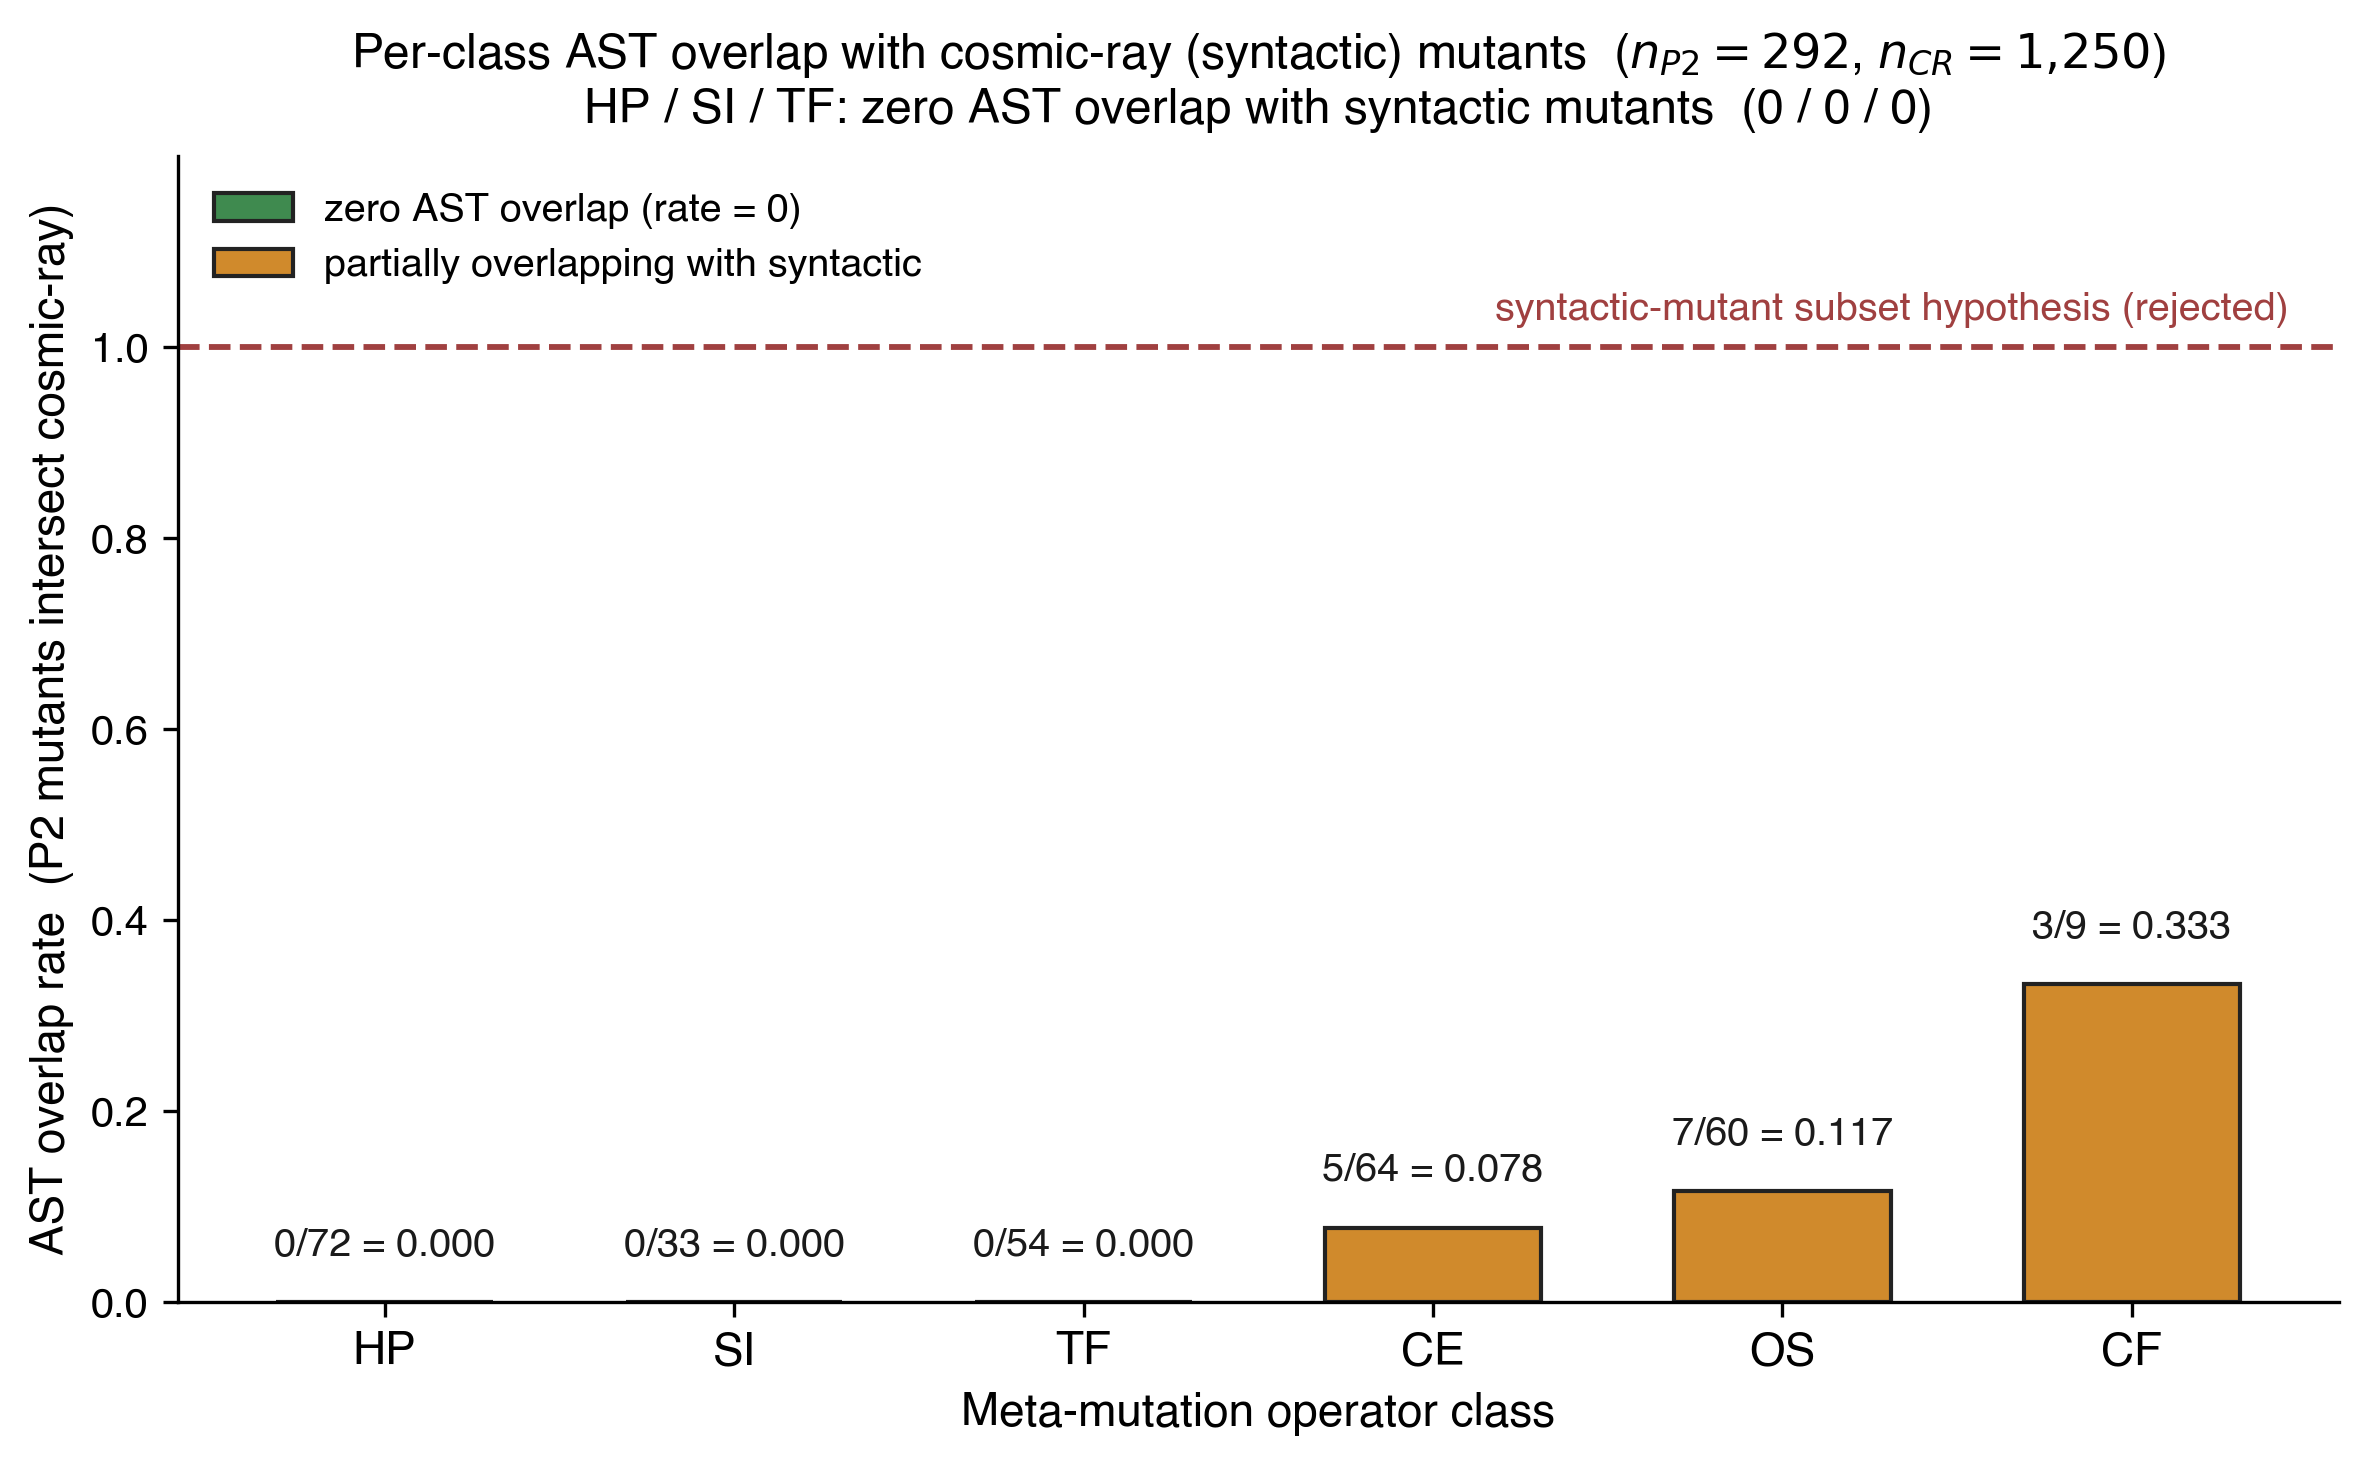
\includegraphics[width=0.8\linewidth,height=\textheight,keepaspectratio]{figures/png/fig3_ast_overlap_per_class.png}
\Description{Bar chart of AST overlap rates by semantic operator family. Hyperparameter, Structural Injection, and Trajectory Flip have zero overlap; Conservation Erosion, Operator Substitution, and the class-specific CF family have nonzero overlap.}
\caption{Per-class AST overlap rate between 292 semantic mutants and 1,250
cosmic-ray syntactic mutants across 12 PUTs (overall 5.14\%). HP, SI, TF
(54.5\% of the semantic pool) show zero overlap (0/72, 0/33, 0/54): SI and TF
are structurally cross-function, while HP zero overlap reflects the
default first-order value menu; CE
7.81\%, OS 11.67\%, CF 33.33\% (CF is a class-specialisation, not in
main 5).}\label{fig:overlap}
\end{figure}

\subsection{Abstract-Syntax-Tree Overlap against Syntactic Mutants}\label{p2-vs-syntactic-mutants-12-put-empirical-layer-3}

\textbf{Experimental design.} For each PUT, semantic cross-source mutants
(\texttt{data/mutants/\$\{PUT\}\_pool\_v4/}, 292 total) are compared at
the AST-normalised level
(\texttt{ast.dump(annotate\_fields=False,\ include\_attributes=False)})
with cosmic-ray default-operator mutants (1,250 total;
\texttt{scripts/p2\_vs\_syntactic\_ast\_diff\_batch.py}). Source:
\texttt{data/results/cosmic\_ray\_12put\_ast\_diff.json}.

\textbf{Aggregate results.} Table~\ref{tab:p2-04} gives the pooled
overlap count.

{%
\begin{longtable}[]{@{}ll@{}}
\caption{Semantic vs syntactic mutants: 12-PUT empirical.}\label{tab:p2-04}\\
\toprule\noalign{}
Metric & Value \\
\midrule\noalign{}
\endfirsthead
\endhead
\bottomrule\noalign{}
\endlastfoot
Total semantic mutants (12 PUTs) & 292 \\
Total cosmic-ray syntactic mutants (12 PUTs) & 1,250 \\
AST-normalised overlap & 15 \\
\textbf{Overall overlap rate} & \textbf{5.14\%} \\
\end{longtable}
}

\textbf{Per-operator-class breakdown (12-PUT aggregate).}
Table~\ref{tab:p2-05} localises that overlap by family.

{%
\begin{longtable}[]{@{}lllll@{}}
\caption{Semantic vs syntactic mutants: 12-PUT empirical.}\label{tab:p2-05}\\
\toprule\noalign{}
Class & n\_p2 & n\_overlap & Rate & Interpretation \\
\midrule\noalign{}
\endfirsthead
\endhead
\bottomrule\noalign{}
\endlastfoot
\textbf{HP} & 72 & 0 & \textbf{0.000} & Structurally unreachable \\
\textbf{SI} & 33 & 0 & \textbf{0.000} & Structurally unreachable \\
\textbf{TF} & 54 & 0 & \textbf{0.000} & Structurally unreachable \\
CE & 64 & 5 & 0.078 & Boundary class (Section~\ref{necessary-conditions-for-semantic-mutation-layer-1} partial (b)) \\
OS & 60 & 7 & 0.117 & Partial incidental hits \\
CF & 9 & 3 & 0.333 & b2 only, n=9 \\
\end{longtable}
}

\textbf{Interpretation: refuting the ``post-classification copy''
challenge.}

\begin{itemize}

\item
  HP, SI, and TF (159 of 292 = 54.5\% of v4 mutants) are
  \textbf{unrepresentable under default first-order configurations} of
  cosmic-ray's AST-local operators such as BinOp, Compare, and
  NumberReplacer. The unreachability is structural under first-order
  operators; whether HOM-based compositions \citep{jia2008subtle} (not
  refuted) can close the gap is a residual higher-order mutation threat, addressed
  conceptually in Section~\ref{preventive-defence-framing}.
\item
  The CE class shows 7.81\% incidental overlap, mostly LLM-generated
  half-step perturbations on a2 and b3 such as
  \texttt{\_RHO=28.0\ $\to$\ 27.5}. The remaining 92.19\% of CE mutants are
  AST-disjoint, because the LLMs prefer domain-aware perturbations over
  integer $\pm$1 changes.
\item
  An earlier draft labelled the OS row ``$\times$ tool-inexpressible''. The
  12-PUT data refines this categorical claim to ``$\bigtriangleup$ 88.33\% disjoint,
  11.67\% incidental hits''. The systematic-versus-incidental argument
  in Section~\ref{preventive-defence-framing} (with details in Appendix B.1) clarifies why those
  incidental hits are stochastic byproducts rather than systematic
  semantic mutation.
\item
  94.86\% of the v4 mutants cannot be reproduced by cosmic-ray defaults.
  The two pools occupy systematically distinct mutant spaces.
\end{itemize}

A multi-tool cross-comparison was not run because mutpy is incompatible
with Python 3.10+, and mutmut's operator set overlaps strongly with
cosmic-ray's. The DeepSeek, Claude, and GPT contributions to the 15
overlap files are uneven (DeepSeek 11, Claude 4, GPT 0). Appendix B.3
covers the cosmic-ray a1 single-PUT pre-12-PUT pilot, and Appendix F
discusses the LLM-source distributional-shift threat.

\subsection{Higher-Order Mutation Boundary}\label{preventive-defence-framing}

The 0/0/0 result for HP, SI, and TF establishes unreachability only for
the tested default first-order configurations. Higher-order mutation
can compose AST-local edits and could approximate some semantic effects;
we did not test that hypothesis and do not claim otherwise
\citep{jia2008subtle,c03829bdd1a6e45113092384bf0fa05a064ca54a,kintis2018effective}.
What the present audit establishes is systematic targeting: the
semantic operators encode cross-boundary, domain-dependent, or
algorithm-class intent and retain provenance labels, whereas incidental
hits by generic operators do not.

Appendix B.6 gives the cosmic-ray/mutmut operator cross-reference and
Appendix F.2 records HOM and LLM-source distribution shift as external
threats. The uneven 15-file overlap (DeepSeek 11, Claude 4, GPT 0) does
not alter the categorical HP/SI/TF zero-overlap result.

\subsection{Adjoint Extension Subjects}\label{adjoint-extension-arm-subjects}

The adjoint invariant $\psi_6$ (Section~\ref{theory-setting}) is exercised on a separate,
confirmatory set of three third-party linear-operator libraries:
scipy \texttt{LinearOperator} (linear algebra), pylops real-FFT (signal
processing), and jax \texttt{linear\_transpose} (automatic
differentiation), disjoint from the 12 PUTs and the pre-registered
60-cell. Each library carries a real fixed defect in its adjoint code
path as a ground-truth anchor (scipy \#8900, pylops \#292, jax \#6223).
For each, the MR families are adj.self (self-adjointness) and adj.dual
(scaled/dual-operator transpose), and the mutant pool mixes
adjoint-breaking mutants (the real defect among them) with semantically
equivalent mutants a strong MR must \emph{not} kill; the real defects are
reproduced in extracted-diff form because the pre-fix releases are
uninstallable on the host (no \texttt{arm64} wheel). The arm is
confirmatory and additive: it does not alter the 60-cell denominator, the
primary-MP convention, or the pre-registered hypotheses. Full subject
specifications and fault mechanisms are in supplementary Appendix H;
results in Section~\ref{rq4-adjoint-extension-arm}.

\subsection{Empirical Study Procedure}\label{procedure-overview}

With the subjects, operators, and the adjoint extension arm fixed
(Sections~\ref{put-selection-12-puts-4-classes}--\ref{adjoint-extension-arm-subjects}), we now specify the procedure that produces each cell's
measurements.

\noindent\textsf{\small Pipeline order: Section~\ref{put-selection-12-puts-4-classes} PUTs $\to$ Section~\ref{cross-source-v4-protocol-summary} Mutant generation $\to$ LRCA L0 prescreen $\to$ Section~\ref{lrca-three-layer-diagnosis} Equivalence ($E_1 \wedge E_2$) $\to$ AVP $\to$ killed/survive $\to$ LRCA three-layer diagnosis $\to$ SMS + $C_1$\_share report.}

Each (i, k) cell is reported with \texttt{inst\_count},
\texttt{equiv\_count}, \texttt{killed\_count}, \texttt{survive\_count},
$\mathrm{SMS}_{i,k}$, $\mathrm{C1\_share}_{i,k}$,
$\mathrm{suspect\_share}_{i,k}$ (the latter two \texttt{NA} on
zero-kill cells), and the
three rates \texttt{inst\_rate\ /\ equiv\_rate\ /\ survive\_rate}
corresponding to RQ3; each admitted mutant additionally carries its
generation-time operator (fiber) label.

\subsection{Cross-Source Generation Protocol}\label{cross-source-v4-protocol-summary}

To isolate the contributions of LLM same-source bias and MR-MP alignment
design to Cliff's delta, we ran a three-stage ablation:
Table~\ref{tab:p2-06} distinguishes the frozen protocol variants.

{%
\begin{longtable}[]{@{}
  >{\raggedright\arraybackslash}p{(\linewidth - 6\tabcolsep) * \real{0.2500}}
  >{\raggedright\arraybackslash}p{(\linewidth - 6\tabcolsep) * \real{0.2500}}
  >{\raggedright\arraybackslash}p{(\linewidth - 6\tabcolsep) * \real{0.2500}}
  >{\raggedright\arraybackslash}p{(\linewidth - 6\tabcolsep) * \real{0.2500}}@{}}
\caption{Cross-source protocol.}\label{tab:p2-06}\\
\toprule\noalign{}
\begin{minipage}[b]{\linewidth}\raggedright
Version
\end{minipage} & \begin{minipage}[b]{\linewidth}\raggedright
Mutant pool
\end{minipage} & \begin{minipage}[b]{\linewidth}\raggedright
c-class primary MP
\end{minipage} & \begin{minipage}[b]{\linewidth}\raggedright
Use
\end{minipage} \\
\midrule\noalign{}
\endhead
\bottomrule\noalign{}
\endlastfoot
\textbf{v3} & Same-source (Claude Opus 4.6) & partial-order (pre-registered) & H2
baseline (pre-registered primary) \\
\textbf{v4} & \textbf{Cross-source} (Claude Opus 4.6 + GPT-5.4 +
DeepSeek chat) & partial-order (held at pre-registered) & Isolate LLM-source
diversity \\
\end{longtable}
}

The v4 protocol (\texttt{scripts/cross\_source\_campaign.py}) runs each
(PUT, operator) pair on Claude / GPT / DeepSeek with K=3 trials under an
identical prompt template (temperature 0.7, V1-V4 mechanical-validation
gate). Cross-source pool capacity: 37 operators $\times$ 3 sources $\times$ 3 trials =
333 attempts, 89.5\% V1-V4 pass, 298 confirmed mutants distributed nearly
equally (Claude 101, GPT 98, DeepSeek 99); final-stage rejection of
duplicate and QA-failing mutants leaves the 292 that enter the v4 pool
used for SMS and the AST audit.
Here ``37 operators'' denotes the executable operator-specialisation
inventory: 36 primary PUT-class operator pairs plus one CF
structural-injection specialisation. The conceptual operator family
count remains five (CE, OS, HP, TF, SI); CF is reported only as a
specialised SI/structural-injection row in the AST-overlap audit.

\textbf{Declared confound: protocol asymmetry.} v3 used the
original Phase-1 dual-blind reviewer protocol (Claude generation +
GPT-5.4 review + DeepSeek arbitration); v4 passes V1-V4 mechanical gates
only and does \textbf{not} invoke a reviewer LLM. A fraction of the v3 $\to$
v4 source-axis contrast may therefore reflect a slight quality shift
rather than LLM-source diversity per se. The follow-up study will rerun
dual-blind on the v4 grid; full per-LLM token / latency / cost figures,
V1-V4 specifications, and the full differential-prompt protocol are in
\textbf{Appendix C.1}.

\subsection{Mutant-pool prescreen and equivalence detection}\label{mutant-pool-prescreen-and-equivalence-detection}

Candidates pass lint/type checks, a finite-output self-test, duplicate
removal, and QA. The v3 pool then uses isolated generator/reviewer LLM
roles plus 20\% manual sampling; v4 uses the V1--V4 mechanical gate and
human C5 review after a kill. This protocol asymmetry is explicit in
Table~\ref{tab:p2-06} and Appendix C.1--C.2.

The operational E1/E2 judgement and killed predicate are defined once in
Sections~\ref{equivalence-judgement-e1-e2-layer-2}
and~\ref{theory-interval}. Here E2 is evaluated first on
\(K_{\mathrm{eq}}=1000\) samples, followed by E1 over the cell's MR
family; E1 and E2 agreement without a certificate is unresolved, while
either failure is confirmed non-equivalence. Each cell uses \(N=20\)
replicates, and the pinned AVP source is embedded in the package.

\subsection{Three-Layer Root-Cause Diagnosis}\label{lrca-three-layer-diagnosis}

For each killed mutant the three-layer decision tree applies in order:

\begin{itemize}

\item
  \textbf{L1 tolerance robustness} (all classes). N=20 replicates with a
  fail-ratio cutoff at 0.80; a kill that survives less than 80\% of the
  20 replicates is labelled C2 (numerical-tolerance perturbation) and
  exits.
\item
  \textbf{L2 OOD triage} (C / D classes only). Sample from
  $\mathcal{D}_P^{\mathrm{valid}}$; if the mutant fails \emph{only} in the OOD
  region, label C3 (out-of-distribution) and exit.
\item
  \textbf{L3 statistical-assumption baseline} (B / D + Wilcoxon / DTW
  only). Pre-check IID / stationarity on the PUT's own repeated samples;
  if the AVP statistical assumption is itself violated, label C4 and
  exit.
\item
  \textbf{Artefact recheck}. An external reviewer re-examines mutant
  code + prompt history; if LLM / artefact evidence (e.g., mutator
  over-injection) is found, label C5; otherwise label C1.
\end{itemize}

Multi-label priority C5 \textgreater{} C4 \textgreater{} C3
\textgreater{} C2 \textgreater{} C1 takes the earliest confirmed
non-semantic cause (decision-tree control flow). The 9-grid scan
($\texttt{ood\_band} \in \{0.02, 0.05, 0.10\}$ $\times$
$\texttt{tolerance\_multiplier} \in \{3.0, 10.0, 30.0\}$, repeats fixed
at 20) calibrates the diagnostic labels only; it does not test H4.
The main analysis retains zero-kill cells as \texttt{NA} and reports
the grid as a post-hoc sensitivity. Detailed grid results, L0--L3
sub-protocols, and decision-tree pseudocode are in
\textbf{Appendix A.2 + C.3}.

% [thematic break removed]

\section{Results and Discussion}\label{statistical-analysis-and-empirical-results}

The empirical thresholds H1--H4 are stress tests of this particular
semantic-mutant instantiation, not prerequisites for the definition of
SMS. The positive validation target is narrower and more structural:
SMS must preserve the mutation-score denominator, separate
domain-semantic mutants from default first-order syntactic mutants, make
MR adequacy failures diagnosable, and distinguish mutant kill-rate,
semantic-stratum alignment, and real-defect detection. Thus the failed
thresholds below are reported as boundary findings about operator
applicability, MR design, and kill attribution; they do not invalidate
the metric construction.

\begin{figure}
\centering
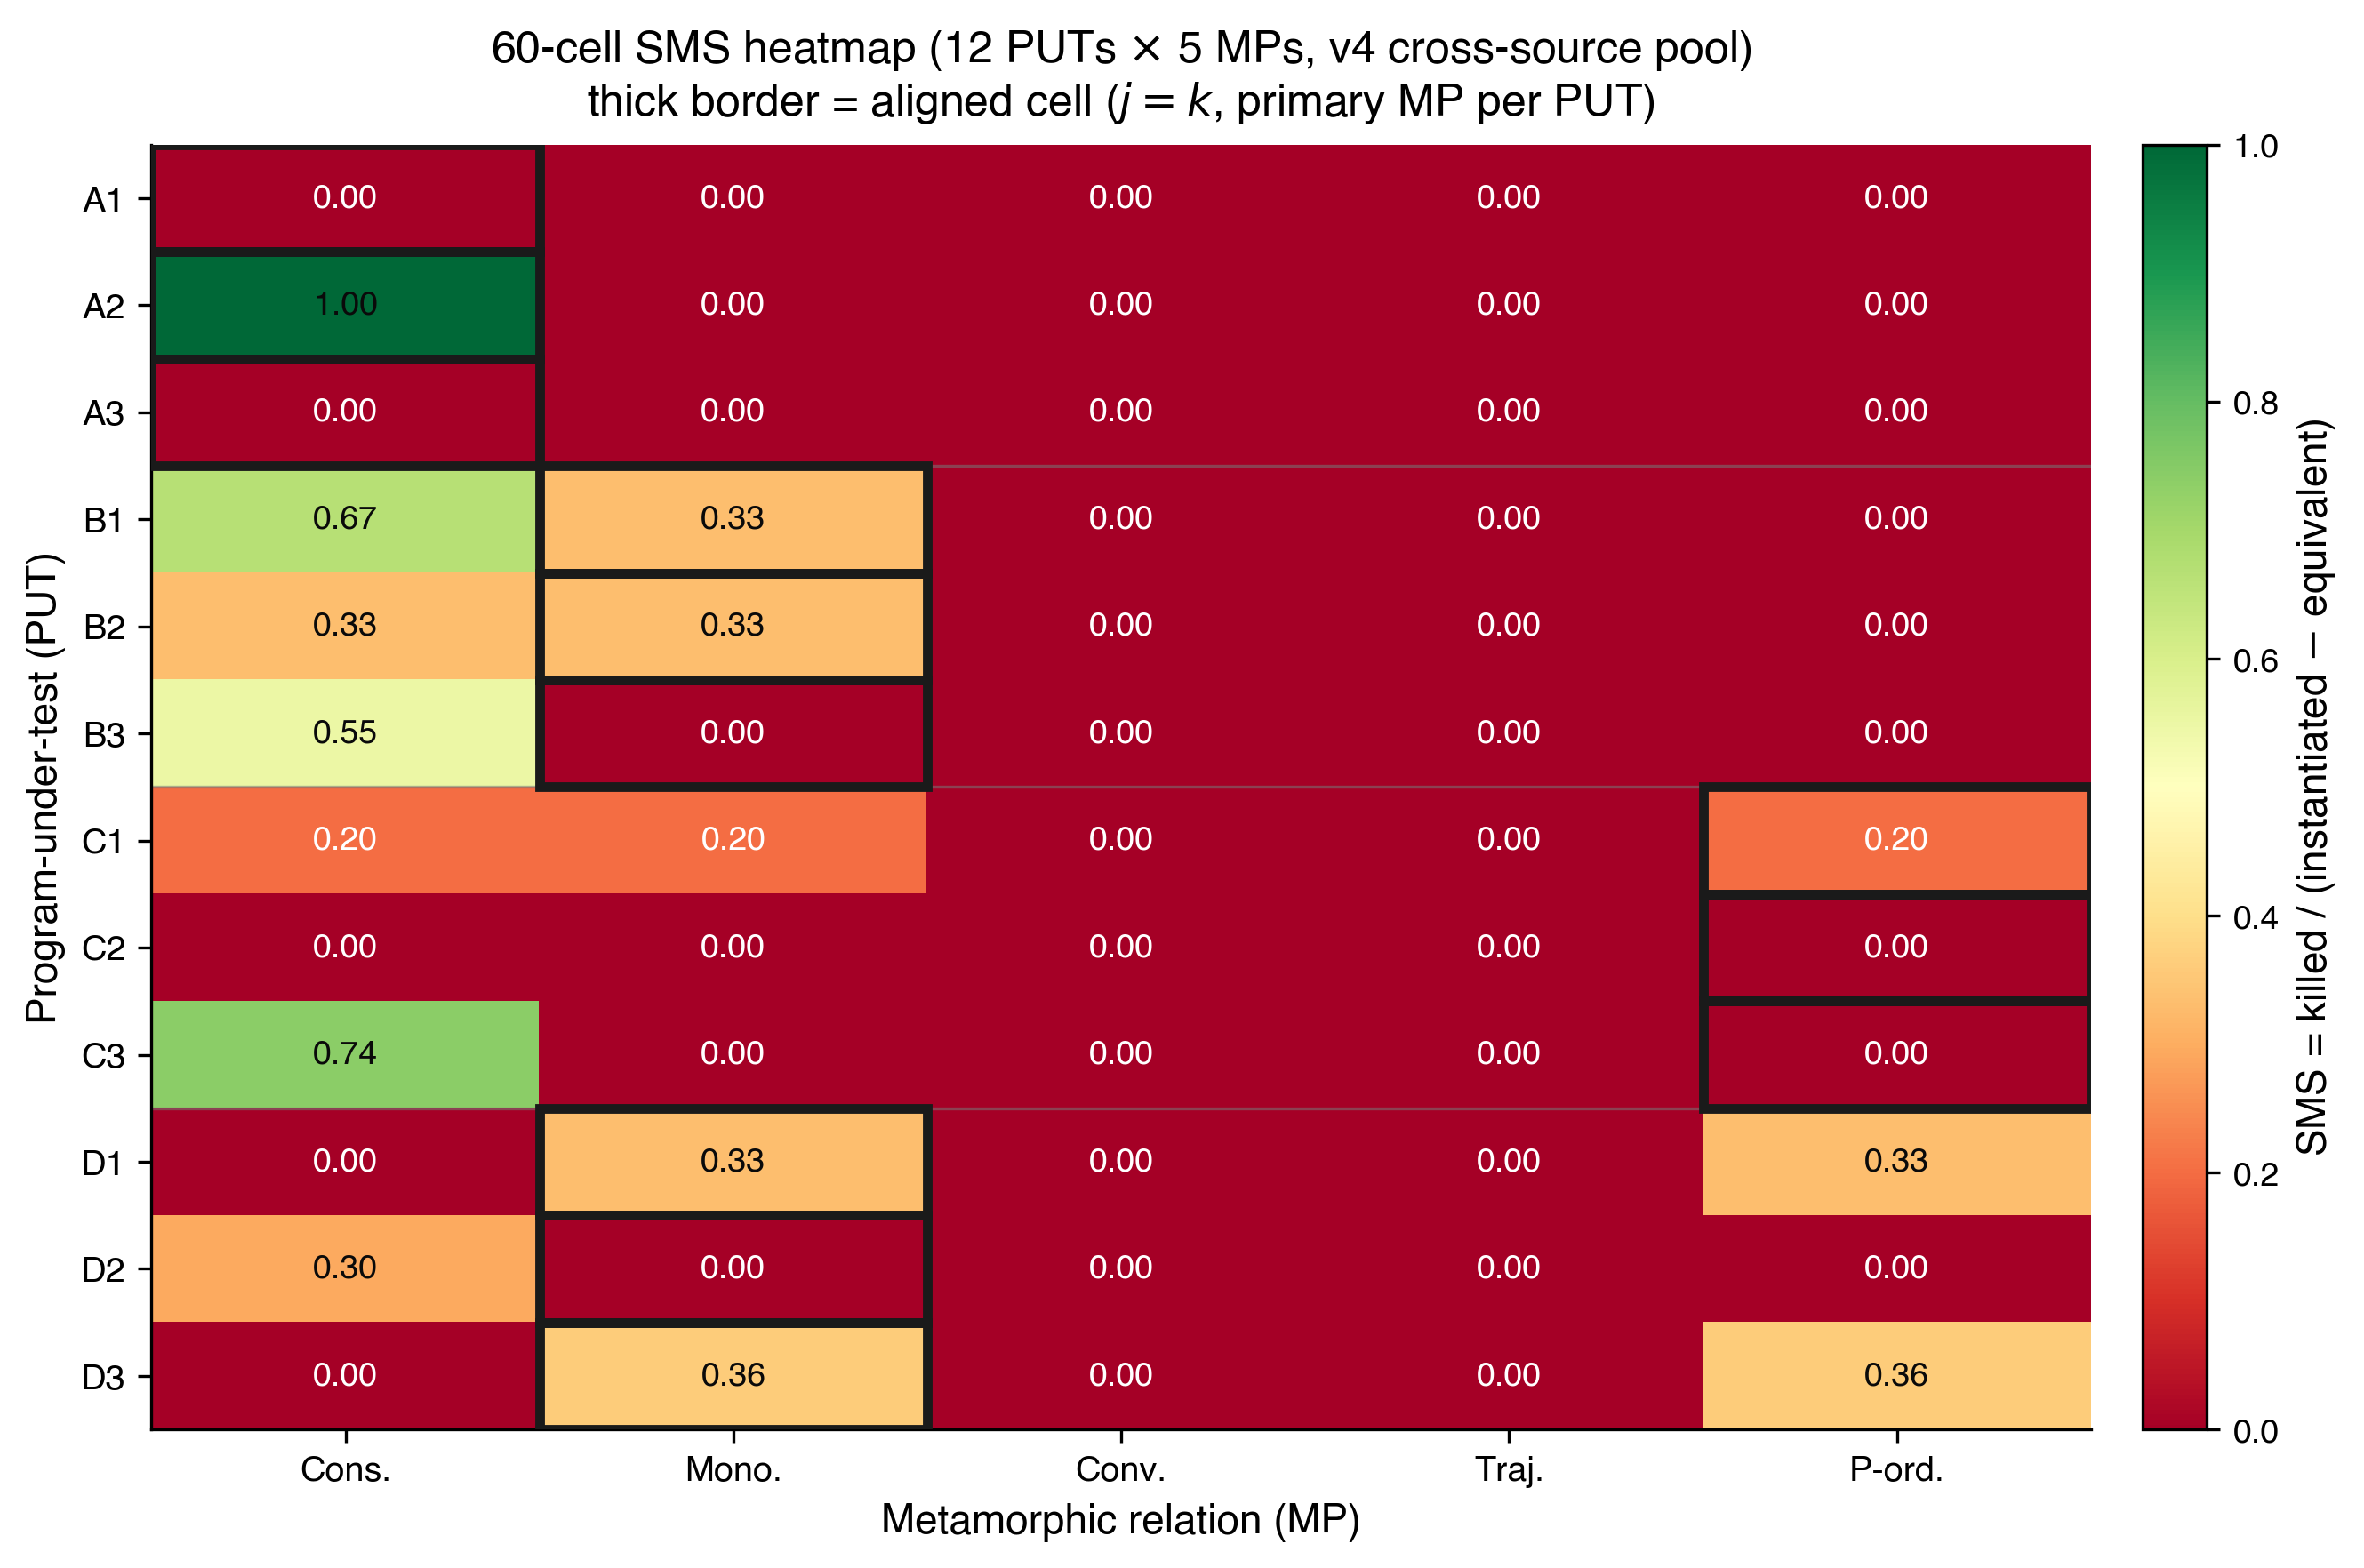
\includegraphics[width=0.9\linewidth,height=\textheight,keepaspectratio,alt={60-cell heatmap of mean SMS over 12 PUTs \textbackslash times 5 MPs (cross-source primary). Diagonal cells (operator-MP aligned) show concentrated mass; off-diagonal mass reflects bleed into adjacent MPs. Empty rows = PUT-level zero-mass cohort (PUTs A1, A3, C2; see Section~\ref{decoupling-between-r_sem-and-r_kill}).}]{figures/png/fig2_60cell_heatmap.png}
\Description{60-cell heatmap of mean SMS over 12 PUTs by five meta-patterns under the cross-source primary pool. Aligned cells concentrate the main signal, while many cross cells are zero; PUTs A1, A3, and C2 form all-zero rows.}
\caption{60-cell heatmap of mean SMS over 12 PUTs \(\times\) 5 MPs (v4
cross-source primary). Diagonal cells (operator-MP aligned) show
concentrated mass; off-diagonal mass reflects bleed into adjacent MPs.
Empty rows = PUT-level zero-mass cohort (PUTs A1, A3, C2; see
Section~\ref{decoupling-between-r_sem-and-r_kill}).}\label{fig:heatmap}
\end{figure}

\subsection{Statistical pipeline}\label{statistical-pipeline}

The primary statistical reporting follows a pre-registered hierarchy:
Table~\ref{tab:p2-07} separates primary from descriptive statistics.

{%
\begin{longtable}[]{@{}
  >{\raggedright\arraybackslash}p{(\linewidth - 4\tabcolsep) * \real{0.3333}}
  >{\raggedright\arraybackslash}p{(\linewidth - 4\tabcolsep) * \real{0.3333}}
  >{\raggedright\arraybackslash}p{(\linewidth - 4\tabcolsep) * \real{0.3333}}@{}}
\caption{Statistical pipeline.}\label{tab:p2-07}\\
\toprule\noalign{}
\begin{minipage}[b]{\linewidth}\raggedright
RQ
\end{minipage} & \begin{minipage}[b]{\linewidth}\raggedright
Primary statistics
\end{minipage} & \begin{minipage}[b]{\linewidth}\raggedright
Reporting format
\end{minipage} \\
\midrule\noalign{}
\endfirsthead
\endhead
\bottomrule\noalign{}
\endlastfoot
RQ3 & inst\_rate, equiv\_rate, C1\_share, survive\_rate & 60-cell
heatmap + 4-class marginals \\
RQ4 & aligned-SMS vs cross-SMS; sparse $\circ$ vs dense \textbullet\textbullet equiv\_rate &
Cliff's delta + odds ratio + 95\% PUT-cluster bootstrap CI \\
RQ5 & $\Delta$SMS\_c (c $\in$ \{A,B,C,D\}); CV($\Delta$SMS) & directional consistency count over the 4 classes (no p-value attached) +
descriptive forest plot \\
RQ5 (desc.) & Spearman $\rho$ + Kendall $\tau$ (SMS vs PC) & scatter + dual-metric ranking
comparison \\
\end{longtable}
}

This pipeline answers the empirical questions RQ3--RQ5; RQ1 is answered
by Theorem~\ref{thm:degeneration} (Section~\ref{sms-ms-degeneration-formal-statement}) and RQ2 by the AST-normalised structural audit
(Section~\ref{p2-vs-syntactic-mutants-12-put-empirical-layer-3}), outside the statistical pipeline.

Where multiple per-class tests are reported (the per-class Friedman tests
of Section~\ref{rq3-cross-class-consistency-and-friedman}), they carry a Bonferroni correction across the four classes; we
do not report a separate cell-level family of p-values, so no family-wise
cell-level correction is claimed. Descriptive cell-bootstrap 95\% CIs
use 1,000 iterations where stated; the headline H2 interval uses
100,000 PUT-cluster resamples (seed 42), preserving each PUT's one
aligned and four cross cells. Mixed-effects
modelling
(\texttt{sms\ \textasciitilde{}\ C(class)\ *\ C(operator)\ +\ (1\ \textbar{}\ put)})
failed with a Singular matrix at N = 60: the class $\times$ operator
interaction design matrix is rank-deficient and the PUT random-intercept
variance collapses to the boundary at this sample size. The Friedman test
is the non-parametric formal alternative. The four hypotheses are
pre-registered: H1 (operator implementability) requires $\geq$ 4 of 5
operators producing $\geq$ 5 non-equivalent mutants on $\geq$ 9/12 PUTs; H2
(aligned-vs-cross) requires odds ratio $\geq$ 3.0 \emph{and} Cliff's delta $\geq$
0.474 (Romano 2006 large-effect threshold); H3 (cross-class consistency)
requires sign-test 4/4 across 4 classes plus CV($\Delta$SMS) \textless{} 0.5;
H4 (LRCA mass) requires mean suspect\_share $\leq$ 0.20 across the 60
cells, an aggregation whose per-cell statistic turns out to be undefined
on zero-kill cells (Section~\ref{h5-lrca-mass}). The primary-table
construction and reporting conventions are in
\textbf{Appendix D.1}.

The results are reported in RQ order. RQ3 is answered in
Section~\ref{rq1-60-cell-distribution}. RQ4 spans the aligned-versus-cross
comparison (Section~\ref{rq2-aligned-vs-cross-cliffs-delta}), its power
analysis (Section~\ref{rq2-stipulated-alternative-power}), the root-cause
diagnostics (Section~\ref{h5-lrca-mass}), the strong-boundary and adjoint
studies (Sections~\ref{rq4-strong-boundary} and~\ref{rq4-adjoint-extension-arm}),
the cross-source analysis
(Sections~\ref{cross-source-contributes-mutant-quality-not-effect-size}
and~\ref{decoupling-between-r_sem-and-r_kill}), and the industrial
construct-separation arm
(Section~\ref{rq4-industrial-construct-separation}). RQ5 follows in
Sections~\ref{rq3-cross-class-consistency-and-friedman}
and~\ref{rq4-sms-vs-pattern-coverage}, with the class-level stability
discussion in Section~\ref{h4-partial-across-same-source-and-cross-source}.

Because the 60 cells share 12 PUTs and are not independent, each
reported statistic carries an explicit inference permission
(Table~\ref{tab:inference-permissions}); no number in this paper should
be read above its row.

{%
\begin{longtable}[]{@{}
  >{\raggedright\arraybackslash}p{(\linewidth - 6\tabcolsep) * \real{0.30}}
  >{\raggedright\arraybackslash}p{(\linewidth - 6\tabcolsep) * \real{0.22}}
  >{\raggedright\arraybackslash}p{(\linewidth - 6\tabcolsep) * \real{0.18}}
  >{\raggedright\arraybackslash}p{(\linewidth - 6\tabcolsep) * \real{0.30}}@{}}
\caption{Inference permissions for the reported statistics.}\label{tab:inference-permissions}\\
\toprule\noalign{}
Statistic & Pre-registration status & Sampling unit (n) & Licensed reading \\
\midrule\noalign{}
\endfirsthead
\endhead
\bottomrule\noalign{}
\endlastfoot
H1 operator--PUT counts & pre-registered threshold & PUT $\times$
operator & deterministic count; verdict factual on this pool \\
H2 Cliff's $\delta$, odds ratio, bootstrap CI & pre-registered
exploratory large-effect target & PUT (n = 12 clusters; each contributes
one aligned and four cross cells) & directional population reading for
this PUT frame from the cluster interval; large-effect verdict remains
the frozen point-estimate rule
(Section~\ref{rq2-stipulated-alternative-power}) \\
H3 sign test, CV($\Delta$SMS) & pre-registered threshold & class (n = 4)
& verdict factual on these four classes \\
H4 mean suspect\_share & pre-registered threshold & cell (evaluable
n = 15 of 60; suspect\_share is \texttt{NA} on zero-kill cells) &
estimand undefined as pre-registered on this data; sensitivity readings
only, no adjudicated verdict \\
Exactness defect $\xi$ (pooled and per cell) & none (descriptive
model-check of Theorem~\ref{thm:gap}) & kill incidence (n = 153) &
descriptive deviation measure under the provenance fiber labels \\
Friedman $\chi^2$ (MP effect; per-class Bonferroni) & exploratory
inferential & PUT blocks (n = 12) & non-parametric alternative after
mixed-effects singularity; exploratory \\
Spearman $\rho$ / Kendall $\tau$ (SMS vs PC) & none (descriptive) & PUT
(n = 12) & hypothesis-generating only \\
Industrial arm: four-group Wilcoxon, Holm-corrected & pre-registered in
the dataset protocol & case (n = 34, paired) & inferential within the
34-case pool; no corpus-level claim \\
Industrial arm: 34/34 real-defect face & none (descriptive; selection-conditioned) & case &
face-level count; not a coverage rate \\
\end{longtable}
}

\subsection{RQ3: Semantic-Mutation Score Distribution}\label{rq1-60-cell-distribution}

{%
\begin{longtable}[]{@{}ll@{}}
\caption{RQ3: Semantic-mutation score distribution.}\\
\toprule\noalign{}
Metric & Value \\
\midrule\noalign{}
\endhead
\bottomrule\noalign{}
\endlastfoot
Number of cells & 60 \\
Mean SMS & 0.104 \\
Median SMS & 0.000 \\
Std SMS & 0.213 \\
Cells with SMS = 0 & 45 / 60 \\
Mean mutants / PUT (v4) & 24.3 (range 10-30) \\
\end{longtable}
}

The \textbf{zero-mass dominance} (45/60 = 75\%) is concentrated in the
cross-MP slice under the frozen primary convention: 81\% (39/48) of
cross cells are zero,
50\% (6/12) of aligned cells are zero. Cliff's delta is
well-defined under this distribution but its inference is effectively
dominated by
\texttt{n\_aligned\_nonzero\ =\ 6\ +\ n\_cross\_nonzero\ =\ 9\ =\ 15}, not the
surface n=60. Median odds ratio is formally infinite (median(cross) =
0); we report ``aligned median \textgreater{} 0 = cross median'' as
auxiliary qualitative evidence. A non-pre-registered binarized
sensitivity uses the odds of nonzero SMS, aligned 6/12 versus cross
9/48, giving an odds ratio of 4.3; we report it only to show that the
ratio criterion's intent survives binarization directionally, not as a
licensed verdict.

\textbf{Effective-n note.} The surface n\_aligned = 12 and n\_cross = 48
mask a much smaller information content: only 15 observations carry
nonzero SMS (6 nonzero aligned + 9 nonzero cross). This is a heuristic
information count, not a formal effective sample size, but it explains the
wide dependence-aware 95\% PUT-cluster interval [0.045, 0.594] of the
v4 primary delta. The implications for power and the H2 verdict direction are
quantified jointly with the stipulated-alternative analysis in Section~\ref{rq2-stipulated-alternative-power}.
PUT-class diversification at n $\geq$ 30 is a testable route to relaxing
the effective-n constraint. Power and effect-size disambiguation are
treated jointly with the stipulated-alternative analysis in Section~\ref{rq2-stipulated-alternative-power}
(avoiding repetition).

\textbf{H1 verdict: not met.} H1 (RQ3) requires at least 4 of the 5
operators to produce $\geq 5$ non-equivalent (confirmed) mutants on at
least 9 of the 12 PUTs. Table~\ref{tab:p2-32} counts confirmed
non-equivalent mutants per operator class across the 12 PUTs in the
audited v4 pool (all 292 admitted mutants are confirmed non-equivalent;
counts from the frozen campaign records): no
operator family clears the $\geq 9/12$ bar, with Hyperparameter closest
at 8 of 12.

{%
\begin{longtable}[]{@{}ll@{}}
\caption{H1: PUTs reaching $\geq 5$ confirmed non-equivalent mutants,
per operator class (v4 pool).}\label{tab:p2-32}\\
\toprule\noalign{}
Operator class & PUTs with $\geq 5$ non-equiv mutants (of 12) \\
\midrule\noalign{}
\endfirsthead
\endhead
\bottomrule\noalign{}
\endlastfoot
Conservation Erosion (CE) & 7 / 12 \\
Operator Substitution (OS) & 7 / 12 \\
Hyperparameter (HP) & \textbf{8 / 12} \\
Trajectory Flip (TF) & 6 / 12 \\
Structural Injection (SI) & 4 / 12 \\
\end{longtable}
}

Because the semantic operators are class-targeted, each is applicable
to a subset of the four PUT classes rather than uniformly to all twelve;
the per-PUT counts are sharply bimodal (a family typically contributes
either a full complement or none on a given PUT). Thus 0 of 5 operators
meet the criterion and \textbf{H1 is
not met as pre-registered}; the uniform-applicability assumption behind
the $\geq 9/12$ bar does not hold for class-targeted operators. An
earlier draft tabulated the operator-level pilot's V1--V4 feasibility
counts here (4/5/9/5/1); those counts measure generation feasibility,
not the pre-registered confirmed-non-equivalent criterion, and are
superseded by the table above.

As a secondary interpretive denominator, we also count only PUTs for
which the operator family has an explicit class-specific specialization
in Appendix B.2 and the operator-level pilot records an attempted
instantiation in Appendix C.3. Under this applicability-adjusted view,
CE reaches 7/8 applicable PUTs, OS 7/7, HP 8/9, TF 6/6, and SI 4/6. The
secondary denominator does not overturn the pre-registered H1 verdict,
but it identifies the scientific source of the failure: within their
intended classes the families are largely implementable, and the
$\geq 9/12$ bar fails because no family is intended to span nine PUTs
except HP. The per-operator implementability profile ($r_{\mathrm{sem}}$,
$d_{\mathrm{impl}}$) is reported in Appendix C.3.

\subsection{RQ4: Aligned and Cross-Pattern Comparisons}\label{rq2-aligned-vs-cross-cliffs-delta}

{%
\begin{longtable}[]{@{}llll@{}}
\caption{RQ4: Aligned and cross-pattern comparisons.}\label{tab:p2-09}\\
\toprule\noalign{}
Slice & n & Mean SMS & Median SMS \\
\midrule\noalign{}
\endhead
\bottomrule\noalign{}
\endlastfoot
aligned ($k = k^\star(i)$) & 12 & 0.213 & 0.100 \\
cross ($k \neq k^\star(i)$) & 48 & 0.077 & 0.000 \\
\end{longtable}
}

The slice statistics are computed under the same frozen primary
convention (c-class at partial order) as the delta point-estimates
below. An earlier draft mixed this table with the withdrawn data-driven
primary configuration (aligned 0.275 / cross 0.061); that configuration
was withdrawn under the permutation null of
Section~\ref{primary-mp-convention} and supports no verdict in this
paper.

Two delta point-estimates under the pre-registered primary-MP
convention are interpreted with the slice summaries in
Table~\ref{tab:p2-09}:

\begin{itemize}

\item
  \textbf{v3 (same-source, pre-registered):} delta = \textbf{0.323}.
\item
  \textbf{v4 (cross-source, c-class held at partial-order):} delta =
  \textbf{0.314}, PUT-cluster 95\% CI [0.045, 0.594]. The cross-source pool
  aggregates Claude / GPT / DeepSeek under an identical prompt; the
  c-class primary is held at the pre-registered partial-order
  meta-pattern so that the v3 $\to$ v4
  contrast holds the prompt and primary-MP choice fixed. Because v4 uses
  mechanical gates rather than the v3 dual-blind reviewer step, the
  source-axis reading is qualified by the protocol-asymmetry analysis in
  Section~\ref{r13-protocol-asymmetry-magnitude-estimate}.
\end{itemize}

\textbf{H2 verdict: not met.} H2 carries two pre-registered criteria,
Cliff's $\delta \geq 0.474$ and an aligned-to-cross odds ratio
$\geq 3.0$. Neither delta crosses the \citet{romano2006cliff}
large-effect threshold 0.474, 0.323 and 0.314 both fall just below the
\citet{romano2006cliff} medium threshold of 0.330, so the delta criterion fails. The
Romano threshold is retained as the frozen decision anchor because it is
the threshold recorded in the experiment design; we do not re-anchor the
verdict post hoc to a Vargha--Delaney interpretation scale. The
odds ratio is degenerate: because the cross-slice median SMS is exactly
0 (table above), the median odds ratio is $+\infty$, so the ratio
criterion is satisfied only trivially under zero-inflation and carries no
evidential weight. H2 is therefore not met as a large-effect target.
The positive PUT-cluster interval supports the directional hypothesis
that aligned MR designs tend to score above cross-pattern designs in
this PUT frame; it does not license a claim that the effect is large. The
contrast $\delta_{\mathrm{v4}} - \delta_{\mathrm{v3}} = -0.009$ (paired-role
bootstrap 95\% CI {[}-0.238, 0.207{]}) is too small to interpret as a stable LLM-source-diversity effect
under the present asymmetric protocol: replacing a same-source pool with
a three-LLM cross-source pool does not appreciably shift Cliff's delta
within this design, but the exact source-diversity contribution requires
a dual-blind v4 rerun.

\textbf{Vacant-cell sensitivity.} Excluding the 9 cells marked vacant in
Table~\ref{tab:p2-cells} gives the same H2 verdict. Under the frozen
primary-MR convention, v4 has n = 11 aligned and n = 40 cross cells,
$\delta = 0.323$ with PUT-cluster 95\% CI [0.045, 0.599].
The direction remains positive and the point estimate remains below
0.474. The sensitivity is a denominator check, not a changed
large-effect verdict.

\subsection{RQ4: Stipulated-Alternative Power Analysis}\label{rq2-stipulated-alternative-power}

The Section~\ref{rq1-60-cell-distribution} effective-n constraint motivates an explicit power analysis. A
plug-in bootstrap (5,000 replications, seed = 42) samples with
replacement from the observed (n = 12, n = 48) v4 SMS distributions. The
bootstrap exceedance-probability table (probability that the resampled
$\hat\delta$ exceeds each threshold under the observed distribution, not
power against a stipulated alternative) is reported in
Table~\ref{tab:rq4-observed-exceedance}:

{%
\begin{longtable}[]{@{}lll@{}}
\caption{RQ4: Bootstrap exceedance probability under the observed
distribution.}\label{tab:rq4-observed-exceedance}\\
\toprule\noalign{}
Threshold & Interpretation & Exceedance prob.\ at (12, 48) \\
\midrule\noalign{}
\endhead
\bottomrule\noalign{}
\endlastfoot
$\delta$ \textgreater{} 0.000 & Any effect & \textbf{0.978} \\
$\delta$ \textgreater{} 0.147 & Small & 0.849 \\
$\delta$ \textgreater{} 0.330 & Medium & 0.457 \\
\textbf{$\delta$ \textgreater{} 0.474} & \textbf{Large (H2)} &
\textbf{0.155} \\
\end{longtable}
}

The plug-in result answers the question ``given the \emph{observed}
distribution, how often do we exceed the threshold?'' A
stipulated-alternative simulation answers a more pointed question: ``if
the \emph{truth} lies at the nearest attainable mixture to the H2
boundary 0.474, how often does the (12,
48) design return $\delta \geq 0.474$?'' SMS distributions have heavy ties at zero
(45 of 60 cells), so a raw shift is discontinuous: any $\varepsilon$ \textgreater{}
0 jumps $\delta$ from 0.314 to 0.74. We therefore use a mixture, drawing the
aligned sample with probability w from (observed\_aligned + 0.001) and
with probability 1 $-$ w from observed\_aligned, calibrating w = 0.373 to
realise $E[\delta] \approx 0.470$; Table~\ref{tab:p2-11} reports the
resulting decision-rule power.

{%
\begin{longtable}[]{@{}lll@{}}
\caption{RQ4: Stipulated-alternative power.}\label{tab:p2-11}\\
\toprule\noalign{}
Stipulated truth & Criterion & Power \\
\midrule\noalign{}
\endfirsthead
\endhead
\bottomrule\noalign{}
\endlastfoot
0.470 (target 0.474) & $\hat{\delta} \geq 0.474$ (point estimate) & \textbf{0.504} \\
0.470 (target 0.474) & Lower 95\% CI bound \textgreater{} 0 (any effect) & 0.895 \\
\end{longtable}
}

The 0.504 result is the expected near-half pass rate for a point
threshold evaluated near its boundary; it does not determine the
source-axis contrast. Sample-size sweeps and the rank-invariance note
are reported once in Appendix D.3.

\subsection{RQ4: Root-Cause Diagnostic Results}\label{h5-lrca-mass}

Table~\ref{tab:p2-13} applies the \texttt{NA} convention consistently.
\begin{table}[t]
\caption{RQ4: Root-cause diagnostic mass under the \texttt{NA}
convention (suspect\_share is undefined on zero-kill cells).}
\label{tab:p2-13}
\centering
\small
\begin{tabular}{ll}
\toprule
Metric & Value \\
\midrule
Cells with at least one LRCA-evaluated kill (v3 / v4) & 12 / 60; 15 / 60 \\
Macro-mean C1\_share (v3; evaluable cells) & 0.821 \\
Macro-mean C1\_share (v4; evaluable cells) & \textbf{0.837} \\
Macro-mean suspect\_share (v4, evaluable cells) & 0.163 \\
Macro-mean suspect\_share (v4, counting L0-prescreened artefact kills as suspect) & 0.186 \\
Pooled suspect kill mass / LRCA-evaluated kills (v4) & 27 / 144 = 0.188 \\
Pooled incl.\ L0 artefact kills (v4) & 36 / 153 = 0.235 \\
Cells with suspect\_share $\leq$ 0.20 (threshold-calibration best, ood\_band = 0.02) & 12 / 15 evaluable (5 aligned + 7 cross) \\
\bottomrule
\end{tabular}
\end{table}

\textbf{H4 verdict: not evaluable as pre-registered.} The
pre-registered criterion is mean suspect\_share $\leq$ 0.20 across the
60 cells. On this data the pre-registered estimand is undefined:
suspect\_share is a share of killed mutants, and 45 of 60 cells have no
kills, so their per-cell statistic is $0/0$. An earlier implementation
coded zero-kill cells as suspect\_share = 1, which produced a reported
mean of 0.791; that number is an artefact of the coding rule, not a
property of the kills (it is dominated by the 45 empty cells), and we
withdraw it. Because every defined aggregation choice is necessarily
post hoc, we render no pass/fail verdict and instead report the
sensitivity range: the evaluable-cell macro-mean is 0.163 (0.186 when
L0-prescreened artefact kills are counted as suspect), the pooled
kill-weighted reading is 0.188 (0.235 incl.\ L0), and 12 of the 15
evaluable cells sit at or below the 0.20 threshold. Under the macro
readings the criterion would hold and under the pooled incl.-L0 reading
it would fail, so the honest summary is that the verdict depends on an
aggregation choice the pre-registration did not fix. The next study
will pre-register pooled suspect kills divided by all LRCA-evaluated
kills as primary and the evaluable-cell macro-mean as secondary, with
zero-kill cells fixed as \texttt{NA}, before observing any outcome. The dense cutoff
sweep of Appendix D.2 is re-based on the evaluable cells accordingly.

\textbf{Exactness-defect audit ($\xi$).} Theorem~\ref{thm:gap} makes
its idealised premises measurable: under the provenance bridge (fiber =
generation-time operator category, CE/OS/HP/TF/SI targeting
$\psi_1$--$\psi_5$; the CF specialisation counts as off-taxonomy), the
pooled exactness defect over the v4 campaign is
$\xi = 117/153 = 0.765$ (\texttt{NA} in the 45 zero-kill cells;
per-cell values in \path{data/results/xi_exactness_defect_v4.json}):
roughly three quarters of kill incidences occur under a checker stratum
different from the killed mutant's generation-time label, and the
diagonal mass concentrates in the CE and OS families. The observable
antecedent of Corollary~\ref{cor:zero} holds in 26/60
cells (6 aligned, 20 cross): 20 have zero SMS and 6 do not. The six
nonzero cases are direct empirical witnesses that the wider
S5/exact-checker premises fail at the provenance-label level. Thus the
block-diagonal decomposition and zero-prediction apply only to the
full-premise subpopulation, not to all 45 observed zero cells. The aligned-cell $\xi$
(0.723) and cross-cell $\xi$ (0.795) are similar, consistent with the
family-boundary and S5-purity slack disclosed in
Section~\ref{decoupling-between-r_sem-and-r_kill}. $\xi$ and LRCA are
complementary: 81\% of LRCA-evaluated kills are C1 (likely semantic),
so most off-fiber kills are genuine semantic detections whose
generation-time label and detecting stratum disagree, evidence of
fiber-label impurity rather than of non-semantic kill mechanisms. $\xi$
is reported alongside SMS and is never folded into it.

\subsection{RQ4: Strong-Boundary Failure Modes}\label{rq4-strong-boundary}

The 60-cell audit (Sections~\ref{rq1-60-cell-distribution}--\ref{h5-lrca-mass}) exercises strong MRs in the regime where
Theorem~\ref{thm:duality} holds. To map the strong boundary of Theorem~\ref{thm:window} we run a
complementary study on six third-party or textbook programs spanning the
meta-patterns, kept separate from the 12 PUTs. Wherever a genuine fixed
defect exists in a third-party library we use real version-switching:
the pre-fix and post-fix releases run unmodified in isolated environments,
and we record the repository, the version pair, and the issue/PR, and
we fall back to a textbook faithful implementation only when the real
defect cannot be exercised on the host (no \texttt{arm64} wheel, a
heavyweight Fortran build, or a drift below machine resolution).
$\varepsilon_{\mathrm{tol}}$ is an explicit factor in every case.
Table~\ref{tab:p2-30} maps the six cases to their boundary roles.

{%
\begin{longtable}[]{@{}p{1.6cm}p{3.4cm}p{2.5cm}p{2.6cm}p{1.7cm}@{}}
\caption{RQ4: Strong-boundary map over six programs.}\label{tab:p2-30}\\
\toprule\noalign{}
Family & Program (provenance; method) & Strong MR ($\varepsilon_{\mathrm{tol}}$) & Correct / faulty verdict & Boundary role \\
\midrule\noalign{}
\endfirsthead
\endhead
\bottomrule\noalign{}
\endlastfoot
inv.con & non-conservative Burgers; \citep{hou1994nonconservative} (textbook) & shock speed ($0.03$) & $0.498$ pass / $-0.002$ killed & strong \\
inv.eqv & scipy \texttt{align\_vectors} $1.13.0\to1.13.1$, \#20660 (real) & rotation residual ($10^{-6}$) & $10^{-16}$ pass / $2.0$ killed & strong \\
adj.self & scipy \texttt{\_adjoint} \#8900/PR\#8962 (real, extracted-diff) & adjoint-identity residual & $10^{-16}$ pass / $1.4$--$2.0$ killed & strong \\
rev.traj & leapfrog vs explicit Euler; \citep{hairer2006geometric} (textbook) & energy-drift ratio ($\leq 3$) & $1.00$ pass / $1952$ killed & strong \\
PINN & soft vs hard BC; DeepXDE \#26 (real torch) & exact BC $|u(0)|$ ($10^{-4}$) & hard $0$ pass / soft $5\times10^{-4}$ flagged (validation reject) & FP (weak MR) \\
struct.\ (FN) & numpy float32 RNG $1.21.6\to1.22.0$, \#17478 (real) & mean / range / dist & both pass; buggy survives & FN (surviving) \\
\end{longtable}
}

\textbf{Strong regime (four cases).} For inv.con, inv.eqv, adj.self, and
rev.traj the correct program satisfies the strong MR within
$\varepsilon_{\mathrm{tol}}$ while the faulty program is killed, exactly
as Theorem~\ref{thm:duality} predicts. Two are real fixed library defects (scipy
\texttt{align\_vectors}; scipy \texttt{\_ScaledLinearOperator.\_adjoint},
whose pre-fix release has no \texttt{arm64} wheel and is therefore
exercised by applying the exact fix diff in reverse); two are textbook
contrasts standing in for a real defect that cannot be exercised on the
host, a conservative versus non-conservative Burgers scheme for the
GeoClaw \texttt{filpatch} conservation bug, and a symplectic leapfrog
versus explicit Euler integrator for the REBOUND IAS15 energy drift, whose
real signature near $10^{-14}$ lies below resolution.

\textbf{False positive, weak MR (PINN).} A physics-informed network
that enforces the boundary condition as a soft penalty is a legitimately
trained, non-faulty model, yet its exact-boundary residual
$|u(0)| \approx 5\times10^{-4}$ exceeds a strict
$\varepsilon_{\mathrm{tol}} = 10^{-4}$, so the exact-boundary relation
flags a correct implementation: the discretisation (the soft
constraint), not a fault, breaks the invariant. Under the killed
predicate such a relation is rejected upstream at MR validation and
contributes no kills (Section~\ref{theory-fibers}); the case is
exhibited as the boundary instance of the weak-MR false-positive remark
of Theorem~\ref{thm:window}, the discrete-program analogue of the
rotational-symmetry counterexample, a continuous invariant reproduced
only approximately. The
hard-constraint ansatz $u = x(1-x)\,\mathrm{NN}(x)$ satisfies the invariant
by construction and passes, confirming that the violation is a property of
the discretisation, not of training.

\textbf{False negative, surviving non-equivalent mutant (RNG).} The
numpy float32 generator defect (\#17478) zeroes the lowest mantissa bit of
every sample; the structural MR family, mean $\approx 0.5$, range
$[0,1)$, distribution shape, is satisfied by both releases within
$\varepsilon_{\mathrm{tol}}$, so the genuinely non-equivalent buggy version
survives. This is coincidental satisfaction of the MR, and because the
fault signature lies below the structural tolerance it is a tolerance
fault; the surviving mutant is non-equivalent (an independent
odd-bit-fraction discriminator reads $0.0$ for the buggy release versus
$\approx 0.5$ for the correct one), and therefore distinct from a
classical equivalent mutant. It is the empirical face of the
stochastic false-negative remark and clause (ii) of
Theorem~\ref{thm:window}: the fault signature sits below the window's
lower edge on the structural observables, and the theorem's repeat
prescription shows why more repetitions cannot recover it there, only a
different observable can.

\textbf{The $\varepsilon_{\mathrm{tol}}$ trade-off.} The PINN case makes
the sensitivity--specificity coupling runnable: at the strict
$\varepsilon_{\mathrm{tol}} = 10^{-4}$ the legitimately-trained soft-BC
model is killed (a false positive), while at a loose
$\varepsilon_{\mathrm{tol}} = 10^{-3}$ it survives correctly; if the same
residual pattern instead arose from a true boundary-condition fault,
loosening $\varepsilon_{\mathrm{tol}}$ would turn that survival into a
false negative. Tightening
$\varepsilon_{\mathrm{tol}}$ trades false negatives for false positives and
loosening it does the reverse, as Theorem~\ref{thm:window} predicts. The strong
boundary is therefore the honest scope of the duality, a tunable
operating point, not a defect to be removed.

\subsection{RQ4: Adjoint Extension Evidence}\label{rq4-adjoint-extension-arm}

Where Section~\ref{rq4-strong-boundary} maps the boundary at which the duality fails, a small
confirmatory arm checks it holding in the forward direction for the sixth
meta-pattern $\psi_6$. On the three third-party linear-operator libraries
of Section~\ref{adjoint-extension-arm-subjects} (scipy, pylops, jax), each carrying a real fixed adjoint defect, a
strong adjoint MR detects only the active mutants: across all three
substrates the correct program survives, every non-equivalent mutant
(including the three real defects scipy \#8900, pylops \#292, and jax
\#6223) is killed, and no semantically equivalent mutant is killed, giving
a forward SMS of 1.00 with zero false positives on the equivalent set
(full subjects, mutant pools, and the per-substrate kill table in
supplementary Appendix H). The arm is confirmatory and additive, it
does not enter the 60-cell denominator and leaves H1--H4 unchanged, and
carries two scope caveats: the scipy \#8900 defect is shared with the Section~\ref{rq4-strong-boundary}
boundary study (so it is not counted as independent corroboration twice),
and the pools are hand-constructed, low-cardinality sets with the real
defects reproduced in extracted-diff form, so the arm demonstrates rather
than measures adequacy (adjoint-arm reproduction-fidelity threat).

% [thematic break removed]

\phantomsection\label{discussion}

\subsection{Cross-source protocol changes diagnostic coverage more than effect size}\label{cross-source-contributes-mutant-quality-not-effect-size}

Going from same-source to cross-source under the pre-registered
primary-MP convention shifts Cliff's $\delta$ by only $-$0.009 (paired-role
bootstrap 95\% CI {[}-0.238, 0.207{]}). LRCA-evaluable cells increase
from 12 to 15 of 60 while their macro-mean C1 share changes from 0.821
to 0.837 (+1.9\% relative); class-c mean SMS rises by \textbf{+91.5\%}, and
class-d mean SMS by 38.3\%. Under an identical prompt template, three
LLMs produce similar distributions for the aligned-vs-cross question.
Within this fixed-prompt but protocol-asymmetric comparison, cross-source
pooling expands diagnostic coverage without materially moving C1 purity
or the aligned-vs-cross effect size. This is a scoped null,
not a general claim that LLM diversity is inert. The strong-sense
source-diversity test, with per-LLM differential prompts (V\_persona,
V\_cot), is deferred to a follow-up study. Appendix C.1 records the full
protocol.

\subsection{Decoupling between Semantic Feasibility and Kill Rate}\label{decoupling-between-r_sem-and-r_kill}

The operator-level pilot in Appendix C.3.1 reveals a sharp pattern: HP,
TF, and OS operators on the c-class (surrogate) and d-class (machine
learning) PUTs reach R\_sem $\approx$ 1.0 (semantic feasibility, the LLM
successfully produces a syntactically valid, executable, intent-bearing
mutant) but R\_kill = 0 under the PUT's primary MP (the AVP fails to
detect the mutant under that MR). Concretely, six cells show R\_sem $\geq$
0.9 with R\_kill = 0: c1\_CE1 (GPR \texttt{noise\_level} 1e-4 $\to$ 1e-1),
c2\_OS1 (polynomial $\to$ spline basis), c3\_HP1 (relu $\to$ tanh), c3\_TF1
(max\_iter 1000 $\to$ 5), d1\_HP1 (MLP $\alpha$ 1e-4 $\to$ 1.0), and d3\_HP1 (LR C 1.0
$\to$ 1e-4). In each, the mutant \emph{is} a valid hyperparameter-semantic
injection, but the primary MP, partial-order (asymptotic) for the
c-class and
monotonicity for the d-class, is an asymptotic or statistical relation,
and the parameter deviation it tolerates is wide enough to absorb the
mutant. We note a family-boundary caveat these examples expose: edits
such as an activation-function swap or an iteration-cap cut sit near
the OS/HP and HP/TF boundaries, and the family label records the
generating operator's intent rather than a unique structural class;
the aligned-versus-cross reading should be taken with this labelling
slack in mind. The same slack exists at the stratum level: S5 purity
(one declared stratum per mutant) is enforced by generation intent and
certificate review, not verified against all five invariants, so part
of the off-diagonal kill mass may reflect multi-stratum effects rather
than pure cross-stratum detection.

The cell-level evidence in Section~\ref{rq1-60-cell-distribution} reproduces this pattern: 75\% of cells
are zero, concentrated in the cross slices. From v3 to v4, LRCA
evaluable cells increase from 12 to 15 while macro C1 share stays high
(0.821 to 0.837). Two observational mechanisms can generate the SMS
pattern: the MR may fail to observe an admitted mutant's effect fiber,
or it may observe that fiber but lack sufficient strength relative to
the tolerance window. The present campaign does not identify a causal
operator effect because \(j\) is a per-mutant generation label rather
than a separately randomized \((i,k,j)\) axis. The positive
aligned-versus-cross contrast therefore supports an MR-design
hypothesis, while the exactness-defect audit of
Section~\ref{h5-lrca-mass} shows that fiber purity is imperfect. Two open questions remain:
whether SMS can infer which MP class is missing for which PUT class, and
whether LRCA can be calibrated with class-specific thresholds separating
likely semantic failures from artefacts.

This decoupling motivates the source-axis reading in
Section~\ref{rq2-aligned-vs-cross-cliffs-delta}: the v3 $\to$ v4
micro-shift of $-$0.009 is descriptive under a fixed prompt and asymmetric
review protocols. A future operator-stratified rerun must restore the
true \((i,k,j)\) axis before operator-level causal claims are tested.

\subsection{RQ4: Industrial Construct-Separation Evidence}\label{rq4-industrial-construct-separation}

The industrial arm answers the last clause of RQ4: whether the
construct separation among aggregate kill-rate, semantic alignment, and
real-defect detection remains visible outside synthetic mutants and
outside author-written kernels. The 34 reproduced, MR-detectable cases
come from the archived dataset \citep{defect4mr2026}
(\href{https://doi.org/10.5281/zenodo.21203424}{10.5281/zenodo.21203424});
dataset construction is not a contribution of this paper.

The pre-registered four-group comparison covers the pattern-derived
relation T1, its ablation A1, literature-generic baselines B1, and seeded
random relations B2. Kill rates are 0.335, 0.310, 0.244, and 0.203,
respectively. T1 exceeds B1 by a mean paired 0.101 (bootstrap 95\% CI
[0.029, 0.179], Holm-adjusted \(p=0.046\), \(\delta=0.247\)); the other
registered comparisons are not significant after correction.

Within the selection-conditioned 34-case face, every tabled defect is
detected by at least one pattern-derived relation; this is not a
corpus-level detection rate. The informative contrast is that B1
detects none in 27 cases, B2 none in 26, and A1 loses 19 detections.
Four non-nesting cases also show generic relations killing mutants that
T1 misses or matches. Thus kill-rate, alignment, and defect detection
remain distinct constructs. Full inclusion rules, case identifiers, and
mechanisms are in supplementary Appendix I.

\subsection{RQ5: Cross-Class Consistency}\label{rq3-cross-class-consistency-and-friedman}

Table~\ref{tab:p2-12} reports the class means and the omnibus
MP-differentiation result.
{%
\begin{longtable}[]{@{}lll@{}}
\caption{RQ5: Cross-class consistency and Friedman statistics.}\label{tab:p2-12}\\
\toprule\noalign{}
Class & Mean SMS (v3) & Mean SMS (v4) \\
\midrule\noalign{}
\endfirsthead
\endhead
\bottomrule\noalign{}
\endlastfoot
a (numeric) & 0.067 & 0.067 \\
b (probabilistic) & 0.156 & 0.148 \\
c (surrogate) & 0.047 & \textbf{0.089 (+91.5\%)} \\
d (ML) & 0.081 & 0.112 (+38.3\%) \\
\end{longtable}
}

Sign test (within-class aligned mean $-$ cross mean, sign = +): \textbf{3
/ 4 (partial) under both v3 (same-source) and v4 (cross-source)}; the
c-class (surrogate) is the inverted cell in both pools ($\Delta$SMS\_c
$= -0.058$ in v3 and $-0.028$ in v4, against $+0.333$ / $+0.093$ /
$+0.149$ for a / b / d in v4).

\textbf{H3 verdict: not met.} H3 carries two pre-registered criteria, a
within-class sign test of 4/4 and CV($\Delta$SMS) $<$ 0.5. The sign test
is 3/4 (partial) under both v3 and v4, cross-source pooling moves the
c-class inversion toward zero ($-0.058 \to -0.028$) but does not
flip it, so the consistency criterion fails. The
per-class effects $\Delta$SMS\_c (aligned mean $-$ cross mean) span from
negative in the inverted class to large positive elsewhere, giving
CV($\Delta$SMS) of 1.10 (v4; 1.36 in v3), far exceeding the 0.5 dispersion threshold,
so the dispersion criterion also fails.

The mixed-effects primary model
\texttt{sms\ \textasciitilde{}\ C(class)\ *\ C(operator)\ +\ (1\ \textbar{}\ put)}
returned Singular matrix; the fallback
\texttt{sms\ \textasciitilde{}\ C(class)\ +\ C(operator)\ +\ (1\ \textbar{}\ put)}
had PUT random-intercept variance hit boundary 0 (degenerate). We
therefore use Friedman as the non-parametric formal alternative:

\begin{itemize}

\item
  \textbf{PUT (n=12) $\times$ MP (k=5), v4 primary pool: chi\^{}2 = 16.76, p = 0.0022}
  (significant; exploratory inferential per Table~\ref{tab:inference-permissions});
  the v3 pool gives the consistent 15.30, p = 0.0041.
\item
  MP rank means (v4): 3.08, 2.58, 2.00, 3.00, 4.33.
\item
  Per-class Friedman with \textbf{Bonferroni $\times$ 4 correction}
  (v4): a 1.000 / b \textbf{0.140} / c 0.924 / d 1.000, no per-class
  result remains significant after correction. Kendall's W effect sizes:
  a 0.333 (small) / b 0.862 (large concordance, but caveat: N=3 per
  class makes this label nominal only) / c 0.467 / d 0.417.
\end{itemize}

\textbf{Caveat.} Friedman tests ``are MP rank differences present''
(averaged over PUTs); H3 tests ``is direction consistent across 4
classes''. These are logically independent. H3 stands on the Section~\ref{rq3-cross-class-consistency-and-friedman} sign
test; per-class Friedman is descriptive only (small N=3 per class).

\subsection{RQ5: Semantic-Mutation Score and Pattern Coverage}\label{rq4-sms-vs-pattern-coverage}

\textbf{Status.} The SMS--Pattern-Coverage relationship, a descriptive
sub-question of RQ5, is reported as a descriptive observation, not a
hypothesis test, because n = 12 places the 95\% Spearman CI at roughly
{[}$-$0.5, +0.6{]}, so the test cannot distinguish zero,
moderate-positive, or moderate-negative correlation. The numbers below
are recorded so that a future study (n $\geq$ 30 PUTs) can pre-register a directional
hypothesis.

Pattern Coverage (PC) per PUT = \#triggered (MP\_k, R\_outcome) cells /
10. Range {[}0.500, 1.000{]}, mean 0.750 (v4). Pairing with mean SMS over 5
MPs: Spearman rho = \textbf{0.163}; Kendall tau = 0.136; n = 12
(descriptive; no inferential reading attaches).

\subsection{Class-Level Stability and Source-Axis Interpretation}\label{h4-partial-across-same-source-and-cross-source}

Cross-source pooling raises the c- and d-class means but does not repair
the c-class inversion or the CV($\Delta$SMS) failure
(Section~\ref{rq3-cross-class-consistency-and-friedman}).

\subsection{Practical Interpretation and Deployment Scope}\label{stakeholder-analysis-single-output-kernels-scope}

\textbf{Scope.} All deployment claims in this subsection are bounded to
single-output \texttt{float\ $\to$\ float} kernels under 2 KB, the 12 PUTs
of this paper. They do not apply to industrial-scale, multi-module, or
multi-output scientific computing software, which lies beyond the scope of this paper.
Table~\ref{tab:sms-lrca-reading} gives interpretive readings for SMS and
LRCA outputs; it is not an acceptance-threshold table.

{%
\begin{longtable}[]{@{}
  >{\raggedright\arraybackslash}p{(\linewidth - 4\tabcolsep) * \real{0.2400}}
  >{\raggedright\arraybackslash}p{(\linewidth - 4\tabcolsep) * \real{0.3800}}
  >{\raggedright\arraybackslash}p{(\linewidth - 4\tabcolsep) * \real{0.3800}}@{}}
\caption{Reading SMS and LRCA together.}\label{tab:sms-lrca-reading}\\
\toprule\noalign{}
Observation & Interpretation & Design response \\
\midrule\noalign{}
\endfirsthead
\endhead
\bottomrule\noalign{}
\endlastfoot
Low SMS, high C1\_share & The MR family detects few mutants, but the
kills it does make are mostly semantic & Add MRs for adjacent semantic
strata before enlarging the mutant pool \\
Low SMS, high suspect\_share & The MR family mainly triggers tolerance,
OOD, statistical, or artefact labels & Inspect tolerances, input domain,
and statistical assumptions before treating kills as adequacy evidence \\
High SMS, low real-defect detection & Mutant kill-rate and defect
detection have diverged & Revisit the declared semantic stratum and add
real-defect-facing MRs \\
Generic relation kills outside the pattern-derived relation & Relation
families are non-nested & Treat the result as a different
semantic-effect fiber, not as domination by one MR family \\
\end{longtable}
}

\textbf{Use.} Test engineers can treat the observed aligned mean 0.213
as a sample descriptor, not a deployment threshold, and use LRCA labels
to choose between MR, tolerance, input-domain, and statistical repairs.
MR designers can run SMS as an offline batch audit; external LLM access,
latency, and non-deterministic cost make it unsuitable for
per-pull-request or regulated air-gapped gating. V\&V documentation may
carry SMS as research evidence alongside code coverage and MR lists,
but no IEC, ISO, ASME, or acceptance-threshold claim is made. Appendix E
contains the workflow, cost, air-gap, and standards details.

All three stakeholder classes consume the same single source of truth
(\texttt{paper\_numbers\_v4.json} and \texttt{lrca\_60cell\_v4.json}) to
avoid documentation fragmentation.

\textbf{Example.} If a surrogate PUT admits a Hyperparameter mutant but
SMS is zero under its primary MR, add a convergence, stability, or
fidelity-order MR before enlarging the mutant pool.

% [thematic break removed]

\section{Threats to Validity}\label{threats-to-validity}

Table~\ref{tab:p2-14} maps each threat to its mitigation and detailed
supplementary treatment.
{%
\begin{longtable}[]{@{}
  >{\raggedright\arraybackslash}p{(\linewidth - 8\tabcolsep) * \real{0.2000}}
  >{\raggedright\arraybackslash}p{(\linewidth - 8\tabcolsep) * \real{0.2000}}
  >{\raggedright\arraybackslash}p{(\linewidth - 8\tabcolsep) * \real{0.2000}}
  >{\raggedright\arraybackslash}p{(\linewidth - 8\tabcolsep) * \real{0.2000}}
  >{\raggedright\arraybackslash}p{(\linewidth - 8\tabcolsep) * \real{0.2000}}@{}}
\caption{Threats to Validity.}\label{tab:p2-14}\\
\toprule\noalign{}
\begin{minipage}[b]{\linewidth}\raggedright
Threat area
\end{minipage} & \begin{minipage}[b]{\linewidth}\raggedright
Threat
\end{minipage} & \begin{minipage}[b]{\linewidth}\raggedright
Class
\end{minipage} & \begin{minipage}[b]{\linewidth}\raggedright
Mitigation summary
\end{minipage} & \begin{minipage}[b]{\linewidth}\raggedright
Detail
\end{minipage} \\
\midrule\noalign{}
\endfirsthead
\endhead
\bottomrule\noalign{}
\endlastfoot
LLM generation & LLM generation reproducibility & Internal & Archived raw responses
+ frozen mutant pools (no user-facing seed; reproducibility by archival) & Appendix F.1 \\
Equivalence approximation & E2 probabilistic approximation & Construct & K\_eq = 1000 +
Hoeffding bound; sweep deferred to future work & Appendix F.1 \\
Shared infrastructure & Shared-infrastructure dependency & Internal & AVP version pinned to the upstream
commit hash; embedded source & Appendix F.1 \\
Root-cause diagnosis & LRCA multi-label boundary & Internal & Decision-tree priority +
multi-label co-occurrence table & Appendix F.1 \\
Representativeness & 12-PUT representativeness & External & shared infrastructure; Appendix B.1
coverage argument; scaling to industrial PUTs & Appendix F.2 \\
Statistical power & Cross-class statistical power & Conclusion & H3 framed exploratory;
Friedman fallback; mixed-effects unavailable & Appendix F.2 \\
LLM homogeneity & LLM homogeneity bias & Construct & 3-LLM rotation + 20\% manual
sampling & Appendix F.2 \\
LLM-source shift & LLM-source distributional shift & External & DeepSeek 11/15 of
overlaps; argument is categorical, not frequency & Appendix F.2 \\
Pool size & Mutant-pool size & Internal & v3 mean 17.4, v4 mean 24.3 per PUT; effect
intrinsic, not pool-dilution & Appendix F.1 \\
LLM non-determinism & LLM non-determinism & Internal & De-dup, K = 10/20 repeats,
raw-response store & Appendix F.1 \\
Higher-order mutation & HOM equivalence & External & Confined claim to first-order
syntactic tools; HOM testing deferred & Appendix F.2 \\
Protocol asymmetry & v3 vs v4 protocol asymmetry (dual-blind reviewer) & Internal &
LRCA evaluable cells 12 $\to$ 15 and macro C1 share 0.821 $\to$ 0.837;
follow-up to rerun
dual-blind on v4 & Appendix F.1 \\
Adjoint reproduction & Adjoint-arm reproduction fidelity and by-construction pools &
Internal & Real defects reproduced through extracted diffs (no
\texttt{arm64} wheel); arm is confirmatory on hand-constructed,
low-cardinality pools, not a high-adequacy discovery; scipy \#8900 is
shared with the Section~\ref{rq4-strong-boundary} boundary study & Section~\ref{rq4-adjoint-extension-arm} \\
Real-defect evidence & Industrial real-defect arm boundary & External & Used at result
level to confirm construct separation; reusable benchmark
construction deferred outside this manuscript & Section~\ref{rq4-industrial-construct-separation} \\
\end{longtable}
}

\textbf{Final limitations.} We list ten known limitations.

\begin{enumerate}
\item
  \textbf{Equivalence determination is a probabilistic approximation.}
  Sampling K\_eq = 1000 inputs is an engineering implementation of the
  undecidable equivalence problem, not a theorem-based decision. A
  Hoeffding-style upper bound on the false-equivalence probability is
  given in supplementary Appendix F.1, but we did not execute a K\_eq sweep over \{500, 1000, 2000\}
  for this submission. A follow-up study will run that sweep.
\item
  \textbf{LLM generation homogeneity bias.} Even with three-LLM
  cross-source pooling, training-data overlap across Claude, GPT, and
  DeepSeek may produce similar blind spots. Three-LLM rotation and 20\%
  manual sampling reduce but do not eliminate this risk. A stronger
  replication should add a fourth, independently trained LLM family; a
  self-hosted open-weight model is the natural candidate.
\item
  \textbf{Limited statistical power for cross-class consistency.} The
  four-class sign test has df = 3, and the mixed-effects model returns
  Singular matrix at N = 60 over 12 PUTs. We treat H3 as exploratory and
  present RQ5 in four pieces: class means, sign test, Friedman, and a
  forest plot.
\item
  \textbf{LRCA reports ``likely'' root causes.} The decision-tree
  priority C5 \textgreater{} C4 \textgreater{} C3 \textgreater{} C2
  \textgreater{} C1 is an engineering choice. The reproducibility
  package preserves the multi-label co-occurrence table for every killed
  mutant as well as the priority-winning root cause; \texttt{root\_cause}
  is best read as a likely cause rather than a definitive causal
  attribution.
\item
  \textbf{The AVP is reused from the shared infrastructure.} Our reproducibility package
  embeds the AVP source code so that the package stays self-consistent under upstream
  evolution, but interface semantics may shift if the upstream infrastructure undergoes a major
  revision.
\item
  \textbf{Epistemological scope versus engineering scope.} SMS measures
  semantic detection capability in the epistemological sense;
  engineering value is not evaluated here.
\item
  \textbf{Signature simplification.} The \texttt{float\ $\to$\ float}
  single-output signature is a substantive constraint, not a purely
  engineering trade-off, and it bounds the upper limit of mutant
  semantic complexity. A portability study should validate SMS on
  industrial-grade multi-output PUTs.
\item
  \textbf{Air-gap incompatibility.} The mutant-generation workflow calls
  external LLM APIs and is incompatible with most regulated air-gapped
  V\&V environments (IEC 60880, DO-178C, IEC 62304, ISO 26262).
  Pre-generated mutant pools can be reproduced offline, but generating
  new pools requires LLM access. Self-hosted open-weight LLMs and
  offline-cached pools are future mitigations.
\item
  \textbf{No proof-carrying semantic-effect certificates.} The present
  workflow admits mutants through E1 $\wedge$ E2, LRCA classification, and
  AST-normalised audit trails. These are empirical and structural
  certificates, not machine-checkable proof objects. In particular, we
  do not yet define an explicit abstraction function from concrete
  program semantics to scientific invariant domains, do not parameterise
  invariant families such as conservation, convergence, and stability as
  abstract-domain elements, and do not attach per-mutant proof, error
  expression, or proof-label certificates that bind a syntactic edit to
  a declared semantic-effect class. This is the main gap between SMS and
  a certificate-bearing semantic mutation framework.
\item
  \textbf{Real-defect evidence is used narrowly.} The industrial
  real-defect arm strengthens this paper's construct argument by showing
  that mutant
  kill-rate, semantic alignment, and real-defect detection can separate
  in practice on reproduced library defects. We do not claim benchmark
  construction, candidate curation,
  repository tooling, or corpus release as contributions of this paper;
  those remain contributions of the archived dataset the arm draws on.
  The semantic-mutant SMS instantiation itself is evaluated on the
  12 controlled kernels only; extending SMS computation to the
  industrial cases is registered follow-up work on the same dataset.
\end{enumerate}

\subsection{Statistical-Modelling Capacity}\label{statistical-modelling-capacity-at-n-60-cells-12-puts}

The mixed-effects primary model
\texttt{sms\ \textasciitilde{}\ C(class)\ *\ C(operator)\ +\ (1\ \textbar{}\ put)}
returned a Singular matrix at N = 60; the fallback
\texttt{sms\ \textasciitilde{}\ C(class)\ +\ C(operator)\ +\ (1\ \textbar{}\ put)}
had the PUT random-intercept variance hit boundary 0 (degenerate). Both
failures are not numerical accidents; rather, they are evidence that 60
observations across 12 PUTs cannot identify an 11-dimensional
fixed-effects structure plus 12-PUT random intercepts. This is a hard
limit of the present design: \textbf{the experiment cannot, in
principle, fit a hierarchical model with this fixed-effect
dimensionality at this sample size}. Friedman tests serve as the
non-parametric formal alternative, but they answer a structurally
different question. Expansion to n\_PUT $\geq$ 30 is the only path to a
properly identified hierarchical model.

\subsection{Programs with Zero Observed Signal}\label{put-level-zero-mass-cohort}

Figure~\ref{fig:heatmap} and Section~\ref{decoupling-between-r_sem-and-r_kill} document that PUTs A1, A3, and C2 produce all-zero
rows across the five MPs in the cross-source pool; that is,
\textbf{for 25\% of the PUTs, SMS gives zero signal at every
cell}. This is a substantive limitation of SMS as an adequacy metric on
this PUT cohort: when the LRCA C1 mass collapses to zero across all
aligned and cross slices for a PUT, SMS cannot distinguish strong from
weak MR sets on that PUT. The phenomenon coexists with R\_sem $\approx$ 1.0
(mutants are valid; Section~\ref{decoupling-between-r_sem-and-r_kill}), so the issue is not mutant generation but
MR-design adequacy at the PUT level. MR-design refinement (per-PUT
MP discovery) and the proposed pre-registered c-class primary-MP rule
on a fresh dataset are the principal mitigation paths. We declare this
as a residual PUT-level zero-signal threat.

\subsection{Protocol-Asymmetry Magnitude Estimate}\label{r13-protocol-asymmetry-magnitude-estimate}

Section~\ref{cross-source-v4-protocol-summary} declared protocol asymmetry: v3 used the Phase-1 dual-blind
reviewer protocol (Claude generation + GPT-5.4 review + DeepSeek
arbitration), while v4 passes V1-V4 mechanical gates only. To quantify
the potential $\delta$-shift attributable to this asymmetry without dual-blind,
we offer a \textbf{rough order-of-magnitude estimate}: in the Phase-1
audit, dual-blind review filtered approximately 5-10\% of LLM-generated
mutants as semantically inconsistent; if these filtered mutants were
systematically less effective at killing under MR\_aligned (a plausible
but unverified premise), the upper-bound $\delta$-shift contribution from
removing the reviewer step is bounded above by approximately
\textbf{$\pm$0.03 to $\pm$0.05 on Cliff's $\delta$} at n\_aligned = 12. This bound is
an order of magnitude larger than the observed $-$0.009 source-axis shift
and therefore prevents reading the source-axis contrast as evidence of
LLM-source-diversity inertness; a direct dual-blind v4 rerun (deferred
to a follow-up study) would give a tighter quantification.

% [thematic break removed]

\section{Future Work}\label{future-work-and-p-series-roadmap}

Seven directions follow from this study.

\begin{enumerate}
\item
  A pre-registered c-class primary-MP rule on a fresh dataset.
\item
  A differential-prompt LLM-diversity test using V\_canonical,
  V\_persona, and V\_cot (full protocol in Appendix C.1.1).
\item
  A scaling study at n $\geq$ 30 PUTs for SMS-vs-Pattern-Coverage
  orthogonality and for HOM-equivalence empirics.
\item
  An abstract-semantics certificate layer: define the observation
  $\mathrm{obs}$ from concrete executions to scientific invariant domains,
  specify CE/OS/HP/TF/SI as semantic-effect predicates over those
  domains, and attach per-mutant proof objects, error expressions, or
  proof labels that certify class membership.
\item
  A rerun of the dual-blind reviewer protocol on the full v4 grid, to
  separate protocol asymmetry from source diversity.
\item
  Cross-language portability work (Python $\to$ JavaScript and Julia)
  building on \citet{tip2025llmorpheus}.
\item
  A self-hosted open-weight LLM pilot for air-gapped industrial
  deployment.
\end{enumerate}

% [thematic break removed]


\section{Conclusion}\label{conclusion}

\subsection{Findings summary}\label{findings-summary}

The pre-registered thresholds stress one instantiation; the metric is
judged by its denominator, guarantees, and auditable evidence interface.

\begin{enumerate}
\item
  SMS preserves the MS ratio while making generation, equivalence, and
  killing relative to declared semantic strata.
\item
  Across 12 PUTs, AST-normalised overlap with default first-order
  mutants is 5.14\%; HP, SI, and TF are 0/72, 0/33, and 0/54.
\item
  Aligned MR designs score above cross-pattern designs in this PUT
  frame: the v4 point estimate is \(\delta=0.314\), with a
  PUT-cluster 95\% CI of [0.045, 0.594]. The direction is supported;
  the pre-registered large-effect point threshold is not met.
\item
  Cross-source pooling shifts \(\delta\) by -0.009 (95\% CI
  [-0.238, 0.207]) while LRCA-evaluable cells increase 12 to 15 and
  macro C1 share changes 0.821 to 0.837.
\item
  MP differentiation is visible (\(\chi^2=16.76\), \(p=0.0022\)), but
  H3 is not met: the class sign test is 3/4 and
  CV(\(\Delta\)SMS) exceeds 0.5.
\item
  In the selection-conditioned industrial face, every tabled defect is
  detected by a pattern-derived relation, while aggregate kill-rate
  advantages are modest and kill sets are non-nested. Kill-rate,
  alignment, and defect detection are distinct constructs.
\item
  H1 is not met; H4 is not evaluable because 45 zero-kill cells make
  its registered cell mean undefined; and \(\xi=0.765\) shows the ideal
  alignment premises are far from exact. These failures identify where
  operator applicability, MR design, and attribution require refinement.
\end{enumerate}

\subsection{Methodological contributions}\label{methodological-contributions}

The three layers are: semantic admission conditions and operator
families; the E1/E2 certificate and classical-MS degeneration; and
AST-normalised empirical traceability. The formal results are auditable
measurement scaffolding---detection-window, interval, and gap
guarantees---while the 60-cell audit is one empirical instantiation.

\section*{Data and Code Availability}\label{data-and-code-availability}

All raw data, mutant pools, AVP source, scripts, and versioned JSON
SSOTs---including \texttt{paper\_numbers\_v4},
\texttt{rq2\_power\_stipulated\_v4},
\texttt{rq2\_cluster\_bootstrap\_v4}, and
\texttt{xi\_exactness\_defect\_v4}---are archived on Zenodo under DOI
\href{https://doi.org/10.5281/zenodo.20250664}{10.5281/zenodo.20250664}.
The industrial real-defect arm (Section~\ref{rq4-industrial-construct-separation}) draws its result-level
statistics from a separately archived defect dataset maintained by the
authors \citep{defect4mr2026}, available on Zenodo under DOI
\href{https://doi.org/10.5281/zenodo.21203424}{10.5281/zenodo.21203424};
benchmark construction and governance are contributions of that dataset,
not of this paper.
An earlier version is available as
\href{https://arxiv.org/abs/2605.17437}{arXiv:2605.17437}. The repository follows
\texttt{REPRODUCIBILITY.md} in the source tree. The cosmic-ray and
mutmut operator versions referenced in Section~\ref{p2-vs-syntactic-mutants-12-put-empirical-layer-3}, Section~\ref{preventive-defence-framing}, and Appendix B.6 are
pinned in \texttt{requirements-frozen.txt}.

% [thematic break removed]


\section*{Supplementary Material}

Appendices A--I (notation and operator catalogue; experimental subjects and
operator specialisations; experimental procedure details; statistical analysis
details; deployment considerations; detailed threats-to-validity mitigation;
the full SMS-to-MS degeneration proof; the adjoint extension arm; and a
result-level real-defect evidence summary) are provided as separate online
supplementary material.

\section*{Funding}

This work was supported by the National Natural Science Foundation of China
(NSFC) General Program (grant no. 12575176); the Hunan Provincial Education
Department Project, China (grant no. 202502000728); the Research Project on
Degree and Graduate Education Reform of the University of South China (grant
no. 2023JG030); the Natural Science Foundation of Hunan Province, China (grant
no. 2025JJ70193); and an industry-funded research project (grant no.
230KHX060001).

\section*{CRediT authorship contribution statement}

\textbf{Meng Li}: Conceptualization, Methodology, Software, Writing, original
draft. \textbf{Xiaohua Yang}: Supervision, Formal analysis, Writing, review
and editing. \textbf{Jie Liu}: Investigation, Validation. \textbf{Shiyu Yan}:
Data curation, Visualization.

\section*{Declaration of competing interest}

The authors declare that they have no known competing financial interests or
personal relationships that could have appeared to influence the work reported
in this paper.

\section*{Generative AI Disclosure}

The authors used AI tools under human direction for editorial proofreading,
LaTeX maintenance, consistency checks, and review-simulation support. All
research claims, methods, experimental data, analyses, and conclusions were
authored, verified, and approved by the human authors.

\bibliographystyle{ACM-Reference-Format}
\bibliography{references}

\end{document}
